\documentclass[
	12pt,
	openright,
	twoside,
	a4paper,
	chapter=TITLE,
	english,
	french,
	spanish,
	brazil
]{abntex2}

\usepackage{estrutura}
\usepackage{helvet}
\usepackage{pdflscape}
\renewcommand{\familydefault}{\sfdefault}

%----------------------------------------------------------------------------- 
% Tamanhos de Fontes
%-----------------------------------------------------------------------------
\renewcommand{\ABNTEXchapterfont}{\bfseries}
\renewcommand{\ABNTEXchapterfontsize}{\large}
\renewcommand{\ABNTEXsectionfont}{\normalfont}
\renewcommand{\ABNTEXsectionfontsize}{\large}
\renewcommand{\ABNTEXsubsectionfont}{\bfseries}
\renewcommand{\ABNTEXsubsectionfontsize}{\large}
\renewcommand{\ABNTEXsubsubsectionfont}{\bfseries}
\renewcommand{\ABNTEXsubsubsectionfontsize}{\large}


% ---
% Dados do documento
% ---

\tipotrabalho{Relatório Técnico}

\titulo{Sistema de apoio à análise de dados com processamento de linguagem natural (NLP)}
% caso não haja, comente a linha abaixo
%\subtitulo{subtítulo (se houver)

\autor{Gustavo da Silva Coelho \\ Raissa Carla Ferreira da Silva}

\orientador{Prof. Me. Giovani Fonseca Ravagnani Disperati}
% caso não haja, comente a linha abaixo
%\coorientador{Prof./Profa. Me./Dr./Dra. Nome Completo}

\curso{Análise e Desenvolvimento de Sistemas}
\grau{Tecnólogo em Análise e Desenvolvimento de Sistemas}

%exemplos
%\curso{Bacharelado em Ciência da Computação}
%\grau{Bacharel em Ciência da Computação em Sistemas para Internet}
%\curso{Especialização em Desenvolvimento de Aplicações para Dispositivos Móveis}
%\grau{Especialista em Desenvolvimento de Aplicações para Dispositivos Móveis}

\campus{Guarulhos}
\area{Área de Concentração do Trabalho}

\local{Guarulhos}
\mes{MÊS}
\ano{ANO}

\instituicao{%
	Instituto Federal de Educação, Ciência e Tecnologia de São Paulo
	\par
	Câmpus \imprimircampus
}

\preambulo{\imprimirtipotrabalho\ apresentado ao Instituto Federal de Educação, Ciência e Tecnologia de São Paulo, como parte dos requisitos para a obtenção do grau de \imprimirgrau.
\\
\\
\\}

\setlength{\parindent}{1.3cm}
\setlength{\parskip}{0.2cm}

\makeindex

% ---------------------------------------------------------------------------------
%                                   INÍCIO DO DOCUMENTO
% ---------------------------------------------------------------------------------
\begin{document}
	
% Seleciona o idioma do documento (conforme pacotes do babel)
%\selectlanguage{english}
\selectlanguage{brazil}

% Retira espaço extra obsoleto entre as frases.
\frenchspacing 


% ---------------------------------------------------------------------------------
%                                   ELEMENTOS PRÉ-TEXTUAIS
% ---------------------------------------------------------------------------------
\pretextual

% ---
% Capa
% ---
%\imprimircapa
% capa personalizada

\begin{center}
	
	%\center
	\large\textsc{\MakeUppercase\imprimirinstituicao}
	\vspace{3.5cm}
	
        \Large\textsc{\imprimirautor}
	\vspace{3.5cm}
	
        \LARGE\textbf{\imprimirtitulo\ifdef{\osubtitulo}{:}{}}
    
    \ifdef{\osubtitulo}{\Large\imprimirsubtitulo}{}
	\vfill
	
	\large\textsc{\imprimirlocal}
	
	\large\textsc{\imprimirano}
	
	\vspace*{2cm}
	
\end{center}

\cleardoublepage


% ---

% ---
% Folha de rosto
% (o * indica que haverá a ficha bibliográfica)
% ---
%\imprimirfolhaderosto*
\begin{center}
   	
   	\Large\textsc{\imprimirautor}
   	\vspace{2.5cm}
   	
        \LARGE\textbf{\imprimirtitulo\ifdef{\osubtitulo}{:}{}}
                           
    \ifdef{\osubtitulo}{\Large\imprimirsubtitulo}{}
   	\vspace{2.5cm}
   	   	
   	\hspace{.4\textwidth}
   	\begin{minipage}{.5\textwidth}
   		\SingleSpacing
   		\large\imprimirpreambulo
   		
   		\vspace{\onelineskip}
   		
   		Orientador: \imprimirorientador
   		
        \ifdef{\ocoorientador}{
     		\vspace{\onelineskip}
   		
    		Coorientador: \imprimircoorientador
        }{}
   		
   	\end{minipage}%
    \vfill
   	
   	\large\textsc{\imprimirlocal}
   	
   	\large\textsc{\imprimirano}
   	
   	\vspace*{2cm}
   	
\end{center}
% ---

% ---
% Inserir a ficha catalográfica
% ---
%
% Este é um exemplo de ficha catalográfica.
%
% A ficha catalográfica final deve ser requisitada pelo aluno e inserida neste
% documento para a entrega da versão final.
%

\begin{fichacatalografica}
    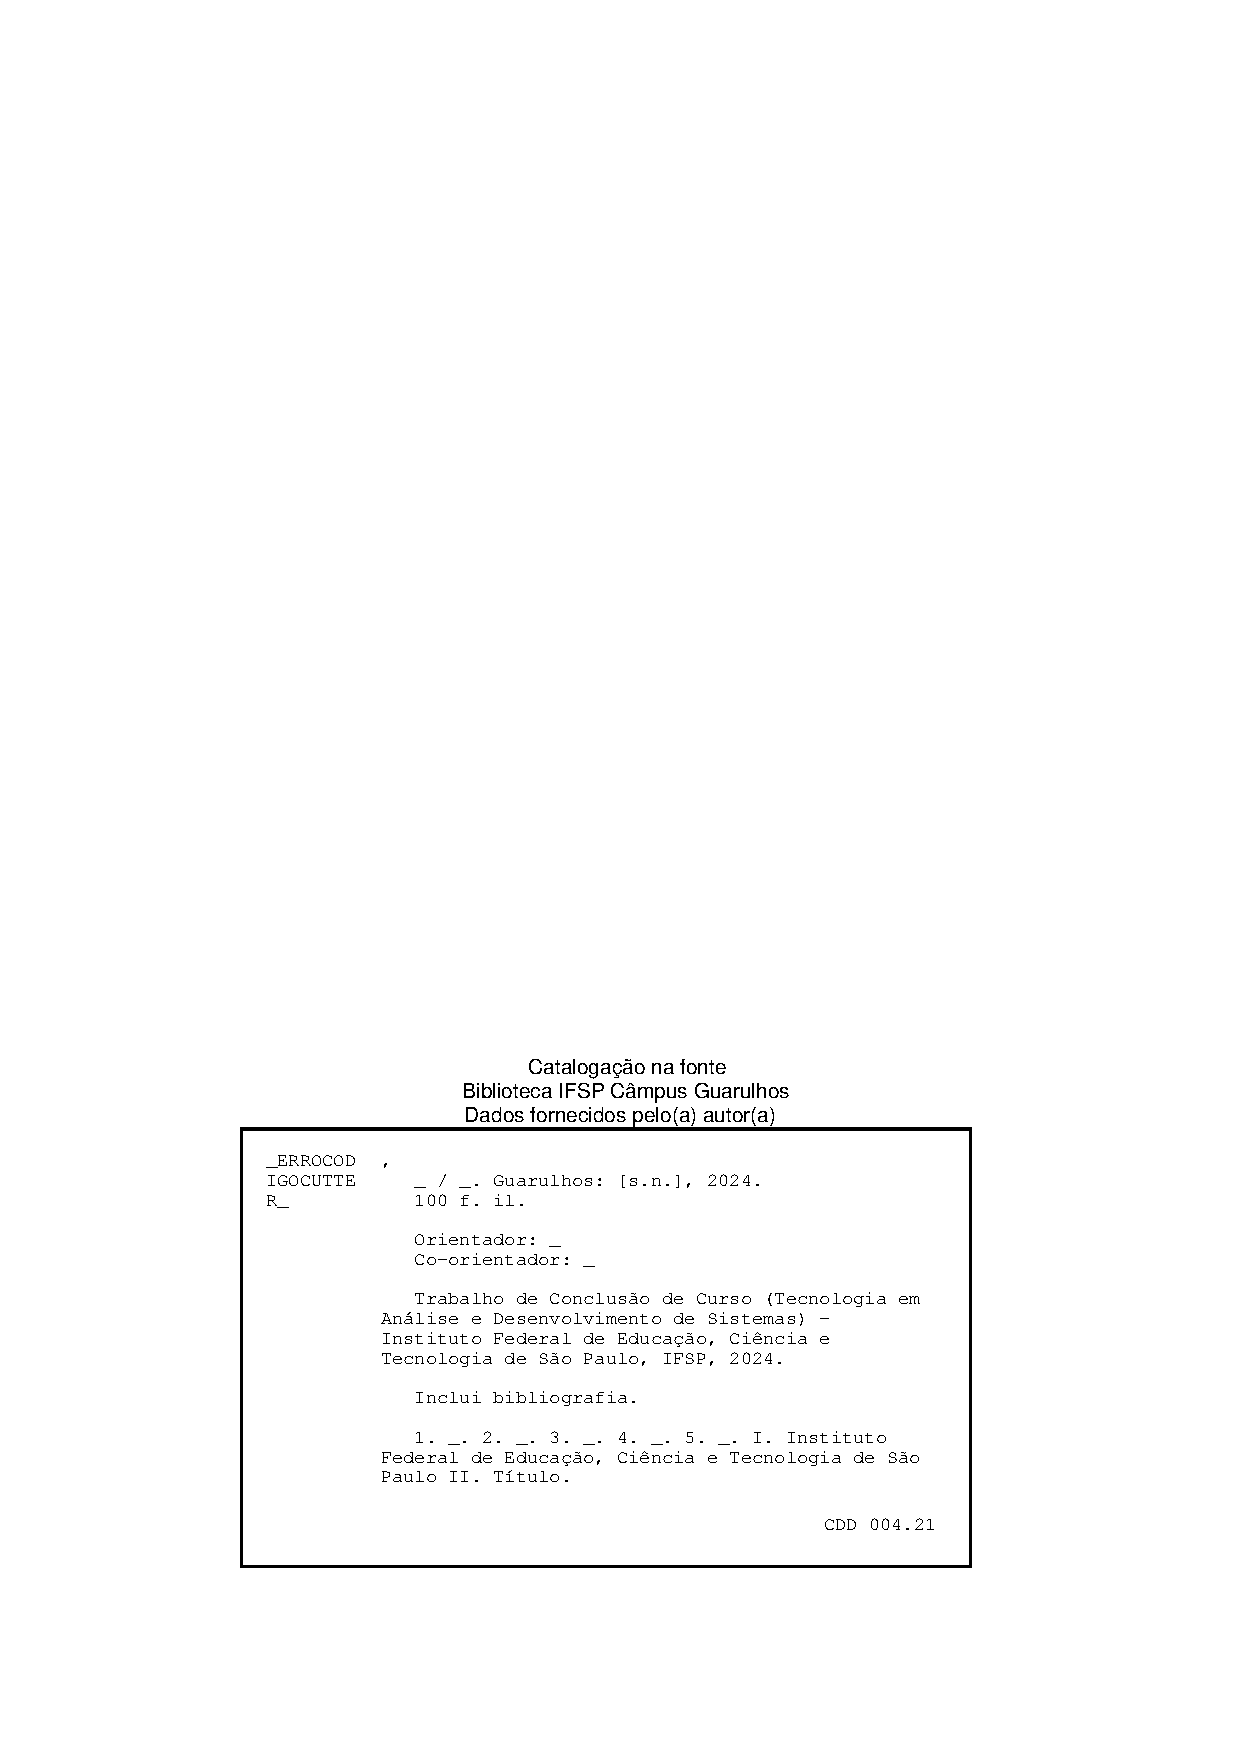
\includepdf{fichaCatalografica/exemploFichaCatalografica.pdf}
\end{fichacatalografica}

% ---
% Inserir ata de defesa
% ---
%
% Este é um exemplo da ata de defesa.
%
% A ata de defesa será fornecida pelo professor orientador após a defesa do trabalho
% e o orientado será responsável em substituir o arquivo de exemplo pelo arquivo final.
%
\begin{folhadeaprovacao}
	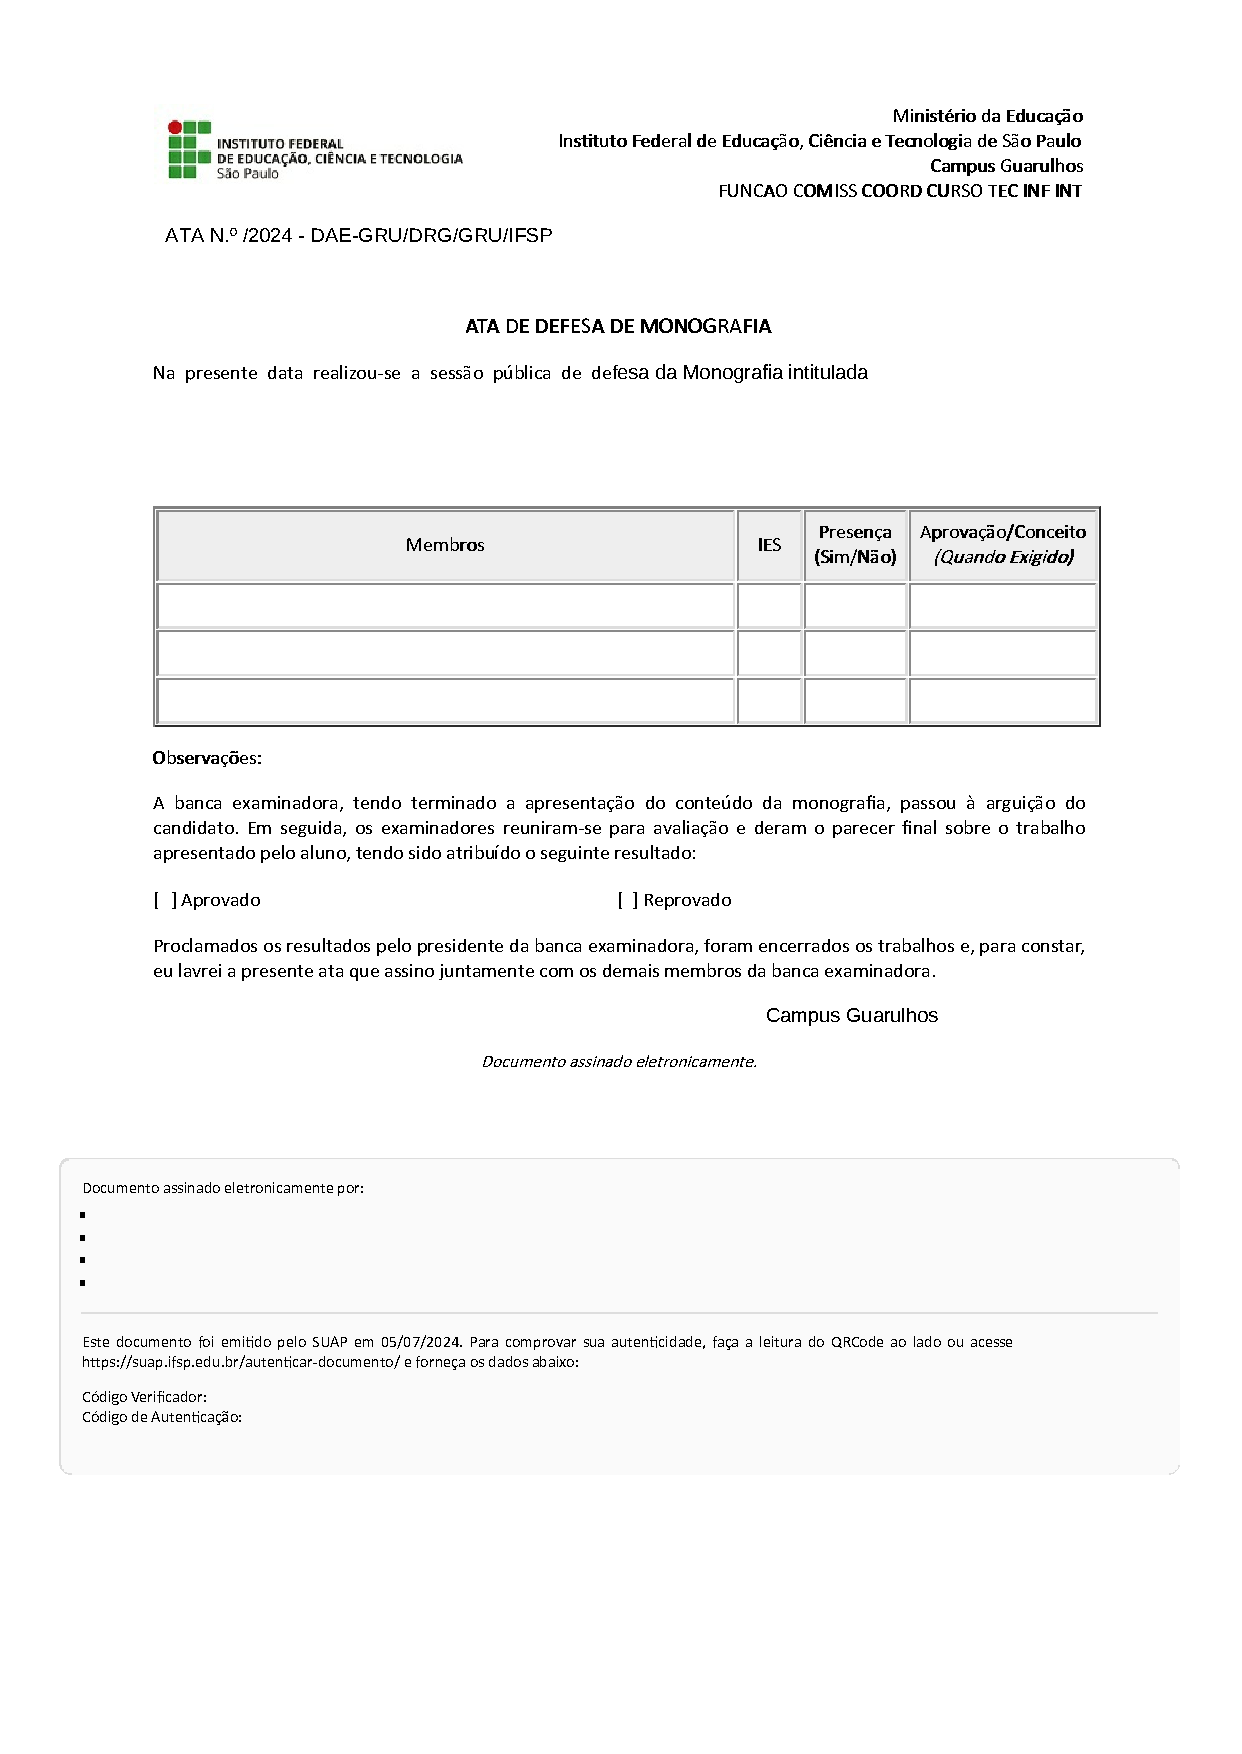
\includepdf[pages={1-}]{ataDefesa/exemploAtaDefesa.pdf}
\end{folhadeaprovacao}

% ---
% Dedicatória
% ---
\begin{dedicatoria}
	\vspace*{\fill}
	\centering
	\noindent
	\textit{Dedicatória (Opcional). Não digite a palavra Dedicatória. Texto no qual o autor do trabalho oferece homenagem ou dedica o seu trabalho a alguém (não usar ponto final)}
    \vspace*{\fill}
\end{dedicatoria}

% ---
% Agradecimentos
% ---
\begin{agradecimentos}
	Agradecimento (opcional). Folha que contém manifestação de reconhecimento a pessoas e/ou instituições que realmente contribuíram com o autor.	
\end{agradecimentos}

% ---
% Epígrafe
% ---
\begin{epigrafe}
	
	\vspace*{\fill}
	Epígrafe (Opcional). Pensamentos retirados de um livro, uma música, um poema, normalmente relacionado ao tema do trabalho, seguida de indicação de autoria. As epígrafes podem ser colocadas também nas folhas de abertura de cada capítulo.  
    
	\epigraph{``\emph{Here's to the crazy ones. The misfits. The rebels. The troublemakers. The round pegs in the square holes. The ones who see things differently. They're not fond of rules. And they have no respect for the status quo. You can quote them, disagree with them, glorify or vilify them. About the only thing you can't do is ignore them. Because they change things. They push the human race forward. And while some may see them as the crazy ones, we see genius. Because the people who are crazy enough to think they can change the world, are the ones who do.}''.}{}
	
\end{epigrafe}

% ---
% Resumos
% ---
\setlength{\absparsep}{18pt} % ajusta o espaçamento dos parágrafos do resumo
\begin{resumo}
	
	Elemento obrigatório, constituído de uma sequência de frases concisas e objetivas, fornecendo uma visão rápida e clara do conteúdo do estudo. O texto deverá conter entre 150 a 250 palavras e ser antecedido pela referência do estudo. Também, não deve conter citações e deverá ressaltar o objetivo, o método, os resultados e as conclusões. O resumo deve ser redigido em parágrafo único, seguido das palavras representativas do conteúdo do estudo, isto é, palavras-chave, em número de três a cinco, separadas entre si por ponto e finalizadas também por ponto. Usar o verbo na terceira pessoa do singular, com linguagem impessoal (pronome SE), bem como fazer uso, preferencialmente, da voz ativa.
	
	\vspace{\onelineskip}
	
	% todas em letras minúsculas, separadas por ponto e vírgula (;)
	\textbf{Palavras-chave}: palavra-chave 1; palavra-chave 2; palavra-chave 3; palavra-chave n.
	
\end{resumo}

% ---
% inserir lista de ilustrações
% ---
\pdfbookmark[0]{\listfigurename}{lof}
\listoffigures*
\cleardoublepage
% ---

% ---
% inserir lista de quadros
% ---
\pdfbookmark[0]{\listofquadrosname}{loq}
\listofquadros*
\cleardoublepage
% ---

% ---
% inserir lista de tabelas
% ---
\pdfbookmark[0]{\listtablename}{lot}
\listoftables*
\cleardoublepage
% ---

% ---
% inserir lista de abreviaturas e siglas
% ---
\begin{siglas}
	\item[1D] Uma dimensão
	\item[2D] Duas dimensões
	\item[3D] Três dimensões
\end{siglas}
% ---

% ---
% inserir lista de símbolos
% ---
\begin{simbolos}
	\item[$\alpha$] Letra grega minúscula Alfa
	\item[$\beta$] Letra grega minúscula Beta
\end{simbolos}
% ---

% ---
% inserir o sumário
% ---
\pdfbookmark[0]{\contentsname}{toc}
\tableofcontents*
\cleardoublepage
% ---






% ---------------------------------------------------------------------------------
%                                  ELEMENTOS TEXTUAIS
% ---------------------------------------------------------------------------------
\textual

\chapter{Introdução} \label{cap:01}

O acesso rápido a informações confiáveis é importante para o acompanhamento de processos e para a tomada de decisões nas organizações. Entretanto, os dados corporativos costumam estar armazenados em bancos de dados relacionais cuja consulta exige conhecimento de linguagens específicas, como a Structured Query Language (SQL). Em consequência, colaboradores que conhecem o contexto do negócio, mas não dominam SQL, frequentemente dependem de profissionais de Tecnologia da Informação (TI) para obter relatórios e responder a perguntas operacionais. Essa dependência pode aumentar o tempo necessário para acessar informações e direcionar a equipe técnica a solicitações repetitivas de extração de dados.

Os avanços em Inteligência Artificial (IA), especialmente no Processamento de Linguagem Natural (PLN), ampliaram as possibilidades de interação entre pessoas e sistemas computacionais. Nesse contexto, a área denominada \textit{text-to-SQL} investiga métodos capazes de interpretar uma pergunta formulada em linguagem natural e transformá-la em uma consulta SQL compatível com a estrutura de um banco de dados \cite{deng2022recent}. Essa abordagem pode tornar a consulta de dados mais acessível, mas ainda envolve desafios relacionados à compreensão da intenção do usuário, à associação entre os termos da pergunta e o esquema do banco, à correção da consulta produzida e à generalização para diferentes estruturas de dados \cite{yu2018spider}.

Este trabalho tem como tema a aplicação de IA na consulta a bancos de dados e delimita-se ao desenvolvimento de uma aplicação desktop para consultas a bancos de dados PostgreSQL. Por meio da plataforma, o usuário poderá formular, em português e sem escrever SQL, perguntas como ``Quais foram os cinco produtos mais vendidos em julho?''. A aplicação enviará a pergunta e as informações necessárias sobre o esquema do banco a um modelo de IA, receberá uma consulta SQL, verificará sua sintaxe e sua segurança, executará apenas consultas de leitura validadas e explicitamente confirmadas pelo usuário e apresentará o resultado de forma compreensível.

O problema que orienta o projeto pode ser expresso pela seguinte questão: como permitir que usuários sem conhecimento técnico em SQL consultem dados relacionais por meio de linguagem natural, preservando a segurança, a integridade e o controle de acesso às informações? Para responder a essa questão, a solução proposta combinará geração de SQL por IA com uma camada de validação independente da resposta do modelo. Serão aceitas exclusivamente consultas do tipo \texttt{SELECT}, e comandos capazes de alterar estruturas ou registros, como \texttt{INSERT}, \texttt{UPDATE}, \texttt{DELETE}, \texttt{DROP}, \texttt{ALTER} e \texttt{TRUNCATE}, deverão ser bloqueados antes da execução.

O MVP contemplará cadastro e login da conta do produto, configuração de conexões PostgreSQL, escolha entre Ollama local e API externa com chave do próprio usuário, histórico local de conversas e apresentação dos resultados em tabelas. A preparação do contexto combinará a estrutura acessível do banco com regras de negócio confirmadas pelo usuário em uma entrevista inicial por conexão. A interface utilizará React, Vite e TypeScript, distribuídos com Electron, e o \textit{back-end} local será implementado em Python com FastAPI. Gráficos, explicações textuais dos resultados, favoritos, sugestões de perguntas e exportações avançadas não integrarão o compromisso da V1. O sistema será avaliado em cenários controlados e com bancos de dados de teste, sem permitir alterações nos dados consultados.

\section{Justificativa}

Sob a perspectiva teórica, o projeto se justifica pela relevância do problema \textit{text-to-SQL} para as áreas de PLN e bancos de dados. A tradução de uma pergunta para SQL não corresponde apenas à substituição de palavras: o sistema precisa identificar a intenção expressa, relacionar entidades e atributos ao esquema disponível e construir uma consulta sintática e semanticamente adequada. A literatura apresenta avanços importantes nessa área, mas também reconhece desafios de interpretação, geração e avaliação das consultas \cite{deng2022recent}. O conjunto de dados Spider, por exemplo, foi elaborado para avaliar consultas complexas e a generalização entre diferentes domínios e esquemas de bancos de dados, evidenciando a necessidade de soluções que sejam testadas além de exemplos simples ou de uma única base \cite{yu2018spider}.

Em termos acadêmicos, o desenvolvimento da plataforma possibilita integrar conhecimentos de engenharia de software, bancos de dados, segurança da informação, desenvolvimento web e IA em um problema aplicado. Além de construir um protótipo funcional, o trabalho permitirá observar em quais tipos de pergunta a geração automática produz resultados corretos, quais erros ocorrem com maior frequência e em que medida as verificações implementadas impedem consultas inadequadas. Assim, a avaliação do sistema poderá produzir evidências sobre as possibilidades e as limitações do uso de modelos de IA como interface para dados relacionais.

Sob a perspectiva prática e de mercado, a solução busca aproximar os dados dos profissionais que precisam utilizá-los, mas que não possuem formação técnica em SQL. Ao permitir consultas em linguagem cotidiana, a plataforma poderá reduzir o tempo gasto em solicitações simples de relatórios, dar maior autonomia aos usuários e liberar a equipe de TI para atividades de maior complexidade. A apresentação tabular, acompanhada da possibilidade de inspecionar a SQL gerada, poderá facilitar a conferência dos resultados e ampliar o uso das informações disponíveis no processo decisório.

Por fim, a adoção de IA nesse contexto exige cuidados específicos, pois uma consulta incorreta pode apresentar resultados enganosos, consumir recursos excessivos ou afetar informações sensíveis. Por esse motivo, a proposta não tratará a resposta do modelo como uma instrução automaticamente confiável. A restrição a operações de leitura, a validação prévia do SQL, o controle de permissões, o registro do histórico e o uso de bancos de teste constituem partes centrais da solução. Dessa maneira, o projeto procura conciliar facilidade de uso e inovação com mecanismos objetivos de segurança e rastreabilidade.

\section{Objetivos}

\subsection{Objetivo Geral}

Desenvolver e avaliar um protótipo de aplicação desktop que permita a usuários sem domínio de SQL consultar bancos de dados PostgreSQL por meio de perguntas em linguagem natural, utilizando IA para gerar consultas de leitura, validando-as e solicitando confirmação explícita antes da execução e apresentando os resultados de maneira segura e compreensível.

\subsection{Objetivos Específicos}

\begin{itemize}
    \item Revisar conceitos, técnicas e trabalhos relacionados a PLN, modelos de IA e conversão de linguagem natural para SQL;
    \item Definir a arquitetura da plataforma e o fluxo de comunicação entre interface desktop, \textit{back-end}, modelo de IA e banco de dados;
    \item Desenvolver uma interface desktop intuitiva com tecnologias web para o envio de perguntas e a visualização das respostas, considerando usuários sem conhecimento técnico em SQL;
    \item Implementar o \textit{back-end} majoritariamente em Python, adotando FastAPI como camada de API local;
    \item Integrar modelos de IA por Ollama local e por API externa do usuário, capazes de gerar SQL a partir de perguntas em português, do esquema autorizado e do contexto de negócio da conexão;
    \item Implementar uma camada independente de validação sintática e de segurança que autorize somente consultas de leitura e bloqueie comandos de alteração de dados ou de estrutura;
    \item Implementar cadastro e login da conta do produto, respeitar as permissões da role PostgreSQL preexistente e persistir configurações e histórico de conversas localmente;
    \item Apresentar a SQL para inspeção e confirmação explícita do usuário e exibir os resultados em tabelas;
    \item Conduzir uma entrevista inicial para registrar regras de negócio validadas em um arquivo de contexto por conexão e permitir a correção controlada de SQL dentro do limite de três tentativas totais; e
    \item Avaliar o protótipo em bancos de dados de teste, considerando a correção das consultas geradas, a efetividade das regras de segurança, o tempo de execução e a compreensão dos resultados apresentados.
\end{itemize}

\chapter{Método de Desenvolvimento}
\label{cap:02}

Este capítulo apresenta o método de desenvolvimento adotado para a construção do sistema proposto, contemplando a visão geral da solução, seus requisitos funcionais e não funcionais, o processo de desenvolvimento de software e as principais tecnologias previstas.

O projeto será conduzido de maneira incremental, priorizando inicialmente a validação do fluxo central da solução: identificação automática da estrutura de um banco de dados PostgreSQL, interpretação de uma pergunta formulada em linguagem natural, geração de uma consulta SQL segura, execução da consulta e apresentação do resultado ao usuário. A partir dessa base, funcionalidades adicionais poderão ser incorporadas progressivamente.

A solução será desenvolvida por uma equipe composta por dois integrantes, utilizando um processo baseado em Kanban e adaptado às características e à escala do projeto acadêmico. O desenvolvimento será acompanhado por meio de um backlog, histórias de usuário, reuniões periódicas e validações progressivas dos incrementos produzidos.


\section{Visão Geral do Projeto}
\label{sec:visao-geral}

O projeto propõe o desenvolvimento de uma aplicação capaz de permitir consultas a bancos de dados PostgreSQL por meio de linguagem natural. O usuário deverá fornecer as informações necessárias para conexão com um banco de dados e, posteriormente, poderá formular perguntas textuais relacionadas aos dados armazenados. A aplicação será responsável por interpretar a solicitação, gerar uma consulta SQL compatível com a estrutura identificada, executá-la de maneira controlada e apresentar o resultado obtido.

Um dos principais componentes da solução será o módulo de descoberta e introspecção do banco de dados, denominado internamente como \textit{crawler}. Esse módulo realizará automaticamente o levantamento da estrutura acessível por meio da conexão fornecida pelo usuário, percorrendo os esquemas disponíveis e identificando, no mínimo, tabelas, colunas, tipos de dados, chaves primárias e chaves estrangeiras.

A descoberta estrutural será realizada de maneira determinística, sem depender diretamente de um modelo de linguagem para identificar os elementos básicos do banco de dados. As informações encontradas serão organizadas em uma representação estruturada e posteriormente utilizadas como contexto pelas etapas responsáveis pela interpretação da solicitação e pela geração da consulta SQL.

Além dos metadados estruturais, o sistema poderá utilizar pequenas amostras dos registros armazenados para auxiliar na compreensão do significado prático das tabelas e colunas. Como essas amostras podem conter informações sensíveis, sua utilização dependerá de consentimento explícito do usuário.

Quando autorizada, a amostragem será limitada a cem registros por tabela, abrangendo todas as colunas acessíveis à role. A autorização será concedida por tabela, com decisão separada para eventual envio a um provedor remoto. Caso o usuário não autorize amostras, o sistema continuará funcionando com os metadados estruturais e o contexto de negócio permitido.

De maneira geral, a arquitetura conceitual da solução será composta pelo seguinte fluxo:

\begin{center}
Interface desktop $\rightarrow$ Preparação do contexto da conexão $\rightarrow$ Geração de SQL $\rightarrow$ Validação independente $\rightarrow$ Inspeção e confirmação pelo usuário $\rightarrow$ Execução somente leitura $\rightarrow$ Resultado tabular.
\end{center}

A aplicação será distribuída como software desktop para Windows, com interface Electron/React e backend Python/FastAPI incluído no instalador e iniciado automaticamente. O núcleo de consulta será executado no computador do usuário, permitindo acesso a PostgreSQL local ou de rede interna. Um serviço separado em nuvem, denominado \textit{Control Plane}, atenderá cadastro, login, registro de contas e instalações e métricas básicas agregadas, sem receber perguntas, SQLs, esquemas, regras de negócio ou resultados. A política de sessão e operação offline desse serviço permanece pendente; sua indisponibilidade não deverá exigir dependência contínua da nuvem para o uso local de Ollama ou da API externa do usuário.

A etapa de interpretação da solicitação também será utilizada para identificar pedidos incompatíveis com o propósito da aplicação. Solicitações que envolvam inserção, atualização, exclusão ou alteração estrutural do banco não deverão prosseguir para execução.

O desenvolvimento será organizado em três marcos de entrega: demonstração de 20\%, prova de conceito V0 e MVP desktop V1. O marco de 20\%, entregue na semana de 2 a 8 de novembro de 2026, demonstrou conexão com PostgreSQL em Docker, introspecção autorizada, geração via Ollama e validação inicial, sem execução da SQL proposta. A V0 está prevista para a semana de 9 a 15 de novembro de 2026, e a V1 para o semestre seguinte.

A \textbf{V0} corresponderá à prova de conceito por interface de linha de comando (CLI), reutilizando o núcleo dos 20\%. Acrescentará contexto de negócio por conexão, até três tentativas totais de geração, confirmação explícita da SQL e execução controlada de leitura com apresentação tabular no terminal. A entrevista poderá ser explorada experimentalmente, sem exigir o fluxo completo da V1.

A \textbf{V1} corresponderá ao Produto Mínimo Viável (MVP) e constituirá a entrega-alvo do trabalho. Integrará o núcleo a uma interface desktop, com múltiplas conexões configuráveis, Ollama local e ao menos uma API externa do usuário, entrevista de contexto por conexão, histórico e configurações locais, proteção opcional de segredos e Control Plane básico. Os resultados serão apresentados em formato tabular.

A \textbf{V2} será considerada uma evolução prevista da solução e acrescentará uma etapa de interpretação dos resultados obtidos, permitindo que o sistema apresente também uma explicação textual dos dados retornados.

Por fim, a \textbf{V3} representará uma evolução voltada à visualização de dados. Nessa etapa, o sistema poderá sugerir formas adequadas de representação gráfica dos resultados, enquanto a interface será responsável pela renderização dessas visualizações.

As versões V2 e V3 serão tratadas como possibilidades de evolução e não como requisitos obrigatórios para a conclusão do MVP.


A unidade de configuração e isolamento será a conexão, incluindo o destino PostgreSQL e a identidade de acesso. Cada conexão terá um único arquivo \texttt{context.md}, com regras de negócio confirmadas pelo usuário. Na V1, a entrevista inicial poderá formular até quinze perguntas, com alternativas sugeridas e resposta livre; hipóteses não confirmadas não serão incorporadas como regras. Na V0, o arquivo poderá ser preparado manualmente.

O \texttt{ContextBuilder} combinará políticas técnicas, esquema autorizado, arquivo de contexto completo, pergunta atual e pares anteriores de pergunta/SQL da mesma sessão. Não haverá RAG, embeddings ou seleção semântica de partes da memória. O orçamento inicial será de oito mil tokens para a memória de negócio e dezesseis mil para o contexto de entrada completo, respeitando a janela do modelo e a reserva de saída; excessos serão informados, sem descarte silencioso de regras. Linhas retornadas por consultas não alimentarão a LLM.

Na V1, o SQLite persistirá apenas dados operacionais locais: perfil e preferências do usuário, configurações de conexões e de IA, consentimentos necessários e histórico de conversas. O conhecimento de negócio permanecerá em Markdown, e senhas e chaves salvas opcionalmente serão protegidas por Electron safeStorage/DPAPI no Windows, com referências no SQLite. Não serão replicados resultados, amostras ou o catálogo completo do PostgreSQL. Na V0, configurações e contexto poderão usar arquivos simples, sem persistência de segredos.


\section{Requisitos}
\label{sec:requisitos}

Os requisitos de software representam os serviços que o sistema deverá oferecer, bem como as restrições que deverão ser consideradas em seu desenvolvimento. Segundo \cite{Sommerville,sommerville2007engenharia}, os requisitos podem ser classificados em funcionais, relacionados diretamente às funcionalidades e comportamentos esperados do sistema, e não funcionais, associados a restrições e propriedades de qualidade da solução.

Além desses requisitos, também será explicitado o não escopo do projeto, delimitando funcionalidades que não serão consideradas parte da entrega prevista. A definição dessas fronteiras contribui para o controle da complexidade e para a manutenção dos objetivos estabelecidos para o projeto \cite{Pressman}.


\subsection{Requisitos Funcionais}

Os requisitos funcionais inicialmente definidos para a aplicação são apresentados a seguir:

\begin{itemize}

    \item \textbf{RF01 -- Conexão com banco de dados:}
    o sistema deverá permitir configurar e testar conexões PostgreSQL com roles preexistentes e permissões restritas, sem provisionamento administrativo; a V1 permitirá manter múltiplas configurações, com uma conexão ativa por conversa.

    \item \textbf{RF02 -- Identificação de esquemas:}
    o sistema deverá identificar automaticamente os esquemas acessíveis utilizando a conexão fornecida.

    \item \textbf{RF03 -- Introspecção estrutural:}
    o sistema deverá identificar automaticamente tabelas, colunas, tipos de dados, chaves primárias e chaves estrangeiras existentes nas estruturas acessíveis.

    \item \textbf{RF04 -- Consentimento para amostragem:}
    o sistema deverá solicitar autorização explícita por tabela para usar amostras, com consentimento separado para envio a um provedor remoto.

    \item \textbf{RF05 -- Limitação das amostras:}
    quando a utilização de registros for autorizada, o sistema deverá limitar a amostragem a cem registros por tabela, incluindo todas as colunas acessíveis à role.

    \item \textbf{RF06 -- Entrada em linguagem natural:}
    o sistema deverá permitir que o usuário formule perguntas sobre os dados utilizando linguagem natural.

    \item \textbf{RF07 -- Validação da intenção:}
    o sistema deverá identificar solicitações incompatíveis com o escopo exclusivamente de leitura da aplicação.

    \item \textbf{RF08 -- Geração de consulta SQL:}
    o sistema deverá gerar consultas SQL de leitura a partir da pergunta, do esquema autorizado e do contexto de negócio validado da conexão ativa.

    \item \textbf{RF09 -- Execução da consulta:}
    o sistema deverá apresentar a SQL validada e executá-la somente após confirmação explícita vinculada à SQL exata e à conexão. A proposta será revalidada antes da execução, em transação somente leitura, com timeout de trinta segundos e limite de linhas; alterações na SQL exigirão nova confirmação.

    \item \textbf{RF10 -- Apresentação do resultado:}
    o sistema deverá apresentar o resultado obtido em formato tabular por meio da interface gráfica da aplicação.

    \item \textbf{RF11 -- Correção automática de consultas:}
    quando uma consulta considerada permitida apresentar falha durante sua geração ou execução, o sistema poderá realizar até três tentativas totais de geração: uma inicial e até duas correções. Cada nova SQL será validada e, para execução, exigirá nova confirmação explícita.

    \item \textbf{RF12 -- Tratamento de falha:}
    caso a consulta não possa ser concluída após o limite de tentativas estabelecido, o sistema deverá encerrar a operação de maneira controlada e informar a falha ao usuário.


    \item \textbf{RF13 -- Contexto de negócio por conexão:}
    o sistema deverá carregar integralmente um \texttt{context.md} por conexão; na V1, uma entrevista de até quinze perguntas permitirá confirmar, corrigir ou rejeitar hipóteses antes de gravar as regras, que poderão ser revistas pelo usuário.

    \item \textbf{RF14 -- Configuração de IA:}
    a V1 deverá permitir configurar e testar perfis de Ollama local e de ao menos uma API externa com chave do próprio usuário.

    \item \textbf{RF15 -- Persistência local:}
    a V1 deverá manter histórico de conversas com perguntas, SQLs e estados de validação, além de preferências, configurações e consentimentos essenciais. Resultados tabulares não integrarão o histórico persistente por padrão.

    \item \textbf{RF16 -- Conta e instalação:}
    a V1 deverá oferecer cadastro e login e registrar conta e instalação no Control Plane, com métricas agregadas que não incluam o conteúdo das consultas ou do contexto.

\end{itemize}

Como requisitos evolutivos, posteriores ao MVP, estarão previstos a geração de explicações textuais sobre os resultados na V2 e a geração ou sugestão de visualizações gráficas na V3.


\subsection{Requisitos Não Funcionais}

Os principais requisitos não funcionais definidos são:

\begin{itemize}

    \item \textbf{RNF01 -- Segurança:}
    o sistema deverá operar exclusivamente com consultas de leitura, bloqueando escrita e alteração estrutural por validação sintática com SQLGlot e política conservadora, combinadas com role de menor privilégio, transação somente leitura, timeout e limites de retorno. A LLM não receberá credenciais nem autoridade de execução.

    \item \textbf{RNF02 -- Privacidade:}
    amostras somente poderão compor o contexto mediante autorização por tabela e consentimento separado para envio remoto. Resultados de consultas não serão enviados à LLM; segredos não serão incluídos em prompts ou logs.

    \item \textbf{RNF03 -- Independência da amostragem:}
    a recusa do usuário em disponibilizar amostras de registros não poderá impedir o funcionamento básico da aplicação, que deverá permanecer capaz de operar utilizando apenas os metadados estruturais do banco.

    \item \textbf{RNF04 -- Modularidade:}
    a arquitetura deverá manter separadas as responsabilidades relacionadas à introspecção do banco, preparação de contexto, geração de SQL, validação, execução e apresentação dos resultados.

    \item \textbf{RNF05 -- Baixo acoplamento ao modelo de linguagem:}
    a integração com inteligência artificial deverá ser projetada de maneira que permita a substituição do modelo ou do provedor sem exigir a reestruturação completa da aplicação.

    \item \textbf{RNF06 -- Tratamento de erros:}
    falhas relacionadas à conexão com o banco, comunicação com o provedor de inteligência artificial, geração da consulta ou execução do SQL deverão ser tratadas de forma controlada.

    \item \textbf{RNF07 -- Observabilidade:}
    o sistema deverá registrar informações suficientes para permitir a análise de seu comportamento durante os testes, incluindo latência, categorias de erro, quantidade de tentativas e estado da execução, sem registrar indiscriminadamente dados pessoais, segredos ou linhas de resultado.

    \item \textbf{RNF08 -- Usabilidade:}
    a V1 deverá disponibilizar uma interface gráfica executável no computador do usuário, permitindo realizar o fluxo principal da aplicação sem necessidade de interação direta com código-fonte ou terminal.

\end{itemize}

Durante a validação da aplicação também serão consideradas métricas relacionadas ao comportamento operacional do sistema. Entre elas estarão a latência entre a solicitação e a resposta, a ocorrência de erros, o volume de consultas processadas e possíveis limitações de recursos.

Devido ao caráter local e à baixa concorrência esperada para o MVP, as métricas de latência e erros possuirão maior relevância inicial. Também serão avaliadas métricas específicas relacionadas à qualidade da solução, tais como taxa de respostas corretas, taxa de execução SQL bem-sucedida, taxa de bloqueio correto de operações proibidas, quantidade de consultas que necessitaram de novas tentativas e número médio de tentativas realizadas.


\subsection{Não Escopo}

Com o objetivo de manter o desenvolvimento compatível com o tempo, tamanho da equipe e objetivos acadêmicos do projeto, algumas funcionalidades serão explicitamente excluídas do escopo obrigatório.

Não fazem parte do escopo do MVP:

\begin{itemize}

    \item inserção de novos registros no banco de dados;

    \item atualização de registros existentes;

    \item exclusão de registros;

    \item criação, alteração ou remoção de tabelas, esquemas ou demais objetos estruturais;

    \item suporte obrigatório a sistemas gerenciadores de bancos de dados diferentes do PostgreSQL;

    \item suporte inicial a bancos de dados NoSQL;

    \item criação de dashboards completos;

    \item treinamento de um modelo de linguagem próprio;

    \item hospedagem do núcleo de consulta em nuvem ou disponibilização da interface como aplicação web pública; o Control Plane básico será um serviço separado da V1;

    \item construção de catálogo semântico relacional ou banco vetorial; o arquivo de contexto validado por conexão fará parte do escopo;

    \item compartilhamento automático de regras entre conexões, consultas federadas e atualização automática do catálogo;

    \item RAG, embeddings, gráficos, explicações textuais de resultados, exportações avançadas, cobrança e API intermediária paga do AskDB.

\end{itemize}

Catálogos semânticos estruturados e mecanismos de recuperação poderão ser avaliados em evoluções posteriores. Essa exclusão não abrange os termos e regras confirmados no arquivo de contexto da conexão, que integram a V0 e a V1.


\section{Processo de Desenvolvimento de Software}

O desenvolvimento da aplicação será realizado utilizando uma abordagem incremental e iterativa, apoiada por um processo baseado em Kanban e adaptado ao tamanho reduzido da equipe e às características acadêmicas do projeto.

A equipe será composta por dois integrantes. Dessa forma, optou-se por um processo com baixa sobrecarga de gestão e documentação, privilegiando visibilidade das atividades, priorização contínua e execução progressiva das funcionalidades.

O trabalho será organizado a partir de um backlog contendo histórias de usuário, atividades técnicas, correções e demais tarefas necessárias para o desenvolvimento. Os itens serão priorizados conforme sua relevância para o funcionamento da solução e serão selecionados de acordo com a capacidade disponível da equipe.

Serão realizadas reuniões semanais para acompanhamento das atividades, identificação de impedimentos, revisão das prioridades e definição dos próximos itens do backlog. O Kanban será utilizado de maneira adaptada, sem a necessidade de introduzir papéis ou cerimônias que não agreguem valor ao contexto de uma equipe composta por apenas dois integrantes.

O desenvolvimento partirá do marco de 20\% já entregue e seguirá para V0 e V1; V2 e V3 permanecerão como possibilidades posteriores. A V0 será utilizada principalmente para reduzir os riscos técnicos relacionados à introspecção do PostgreSQL, preparação de contexto, geração de consultas SQL e execução segura. Após a validação desse fluxo, o projeto avançará para a V1, correspondente ao MVP e à principal entrega prevista no TCC, incluindo a integração do backend com uma interface gráfica.

Essa organização também se relaciona com os princípios de customização de processos, ou \textit{tailoring}, estudados durante a disciplina. A implementação gradual de um processo ou solução permite que áreas prioritárias sejam tratadas primeiro, evitando a tentativa de implantação de todos os elementos simultaneamente. No contexto deste projeto, essa ideia será aplicada por meio da divisão da solução em incrementos progressivos, nos quais cada versão adicionará novas capacidades a uma base previamente validada.

Outro princípio considerado será a seleção de artefatos de acordo com o valor que fornecem ao desenvolvimento. Considerando o tamanho da equipe, serão priorizados os documentos e artefatos necessários para apoiar a comunicação, rastreabilidade, implementação e avaliação da solução, evitando a produção de documentação cujo custo de elaboração e manutenção não seja proporcional ao benefício obtido.

Entre os principais artefatos previstos encontram-se:

\begin{itemize}

    \item backlog do produto;

    \item histórias de usuário;

    \item especificação de requisitos;

    \item documentação da arquitetura;

    \item diagramas considerados necessários para representar a solução;

    \item código-fonte versionado;

    \item casos e resultados de testes;

    \item relatório técnico do projeto.

\end{itemize}

A divisão de responsabilidades também será adaptada às características da equipe. Ambos os integrantes participarão do desenvolvimento, especialmente das atividades relacionadas ao backend e ao fluxo central da aplicação. Entretanto, um dos integrantes terá maior concentração nas atividades de organização, documentação e apresentação do projeto, enquanto o outro terá maior concentração na implementação.

Essa divisão não será rígida, e as principais decisões técnicas e atividades de desenvolvimento permanecerão compartilhadas entre os integrantes. Dessa forma, a distribuição de responsabilidades poderá ser representada por uma matriz simplificada, evitando a criação de uma estrutura organizacional desnecessariamente complexa.

O código-fonte será versionado utilizando Git e armazenado em um repositório no GitHub. O versionamento permitirá o acompanhamento das alterações realizadas, a integração do trabalho dos dois integrantes e a recuperação de versões anteriores quando necessário.

A validação do sistema ocorrerá progressivamente durante o desenvolvimento. Será criado um conjunto controlado de perguntas cujos resultados esperados sejam previamente conhecidos, permitindo avaliar o comportamento do sistema diante de diferentes níveis de complexidade.

A avaliação priorizará a correção do resultado retornado, e não necessariamente a igualdade textual entre o SQL produzido pelo sistema e uma consulta de referência. Essa decisão considera que consultas SQL sintaticamente diferentes podem produzir resultados semanticamente equivalentes.

Entre as principais métricas previstas para a avaliação estão:

\begin{itemize}

    \item taxa de respostas corretas;

    \item taxa de consultas SQL executadas com sucesso;

    \item taxa de bloqueio correto de operações proibidas;

    \item quantidade de consultas que exigiram uma ou mais tentativas de correção;

    \item número médio de tentativas realizadas;

    \item latência entre a solicitação do usuário e a apresentação do resultado;

    \item quantidade de tokens utilizados, quando essa informação for disponibilizada pelo provedor;

    \item custo estimado por consulta, quando aplicável.

\end{itemize}

A comparação entre diferentes modelos de linguagem poderá ser realizada internamente durante o desenvolvimento para apoiar a escolha da alternativa que apresente melhor equilíbrio entre qualidade, custo e latência. Entretanto, essa comparação não será considerada, inicialmente, um experimento formal do TCC.


\section{Tecnologias}

A seleção das tecnologias previstas para o desenvolvimento foi orientada pela compatibilidade com o problema proposto, maturidade das ferramentas, facilidade de integração, disponibilidade de bibliotecas e conhecimento prévio da equipe.

A solução será estruturada em duas camadas principais de execução: uma aplicação responsável pela interface com o usuário, construída com React, Vite, TypeScript e Electron, e um backend desenvolvido em Python e FastAPI, responsável pela lógica de negócio, introspecção do banco de dados, integração com modelos de linguagem, validação e execução das consultas.


\subsection{Python}

Python será utilizado como principal linguagem de programação do backend. A linguagem possui um amplo ecossistema de bibliotecas voltadas à integração com bancos de dados, construção de APIs, manipulação de dados e comunicação com modelos de linguagem, características diretamente relacionadas às necessidades da aplicação.

Além disso, sua utilização permitirá concentrar no mesmo ambiente as etapas de introspecção do banco, preparação de contexto, integração com provedores de inteligência artificial e execução das consultas.


\subsection{FastAPI}

O FastAPI será utilizado para a construção da camada de API e para a orquestração dos diferentes módulos do sistema.

O framework será responsável por disponibilizar os serviços utilizados pela interface, receber as solicitações dos usuários e coordenar etapas como conexão com o banco, introspecção, processamento da pergunta, comunicação com o modelo de linguagem e execução das consultas.


\subsection{Pydantic}

O Pydantic será utilizado para definição e validação das estruturas de dados utilizadas pela aplicação.

Sua utilização permitirá estabelecer contratos explícitos para entradas e saídas da API, contribuindo para a validação dos dados recebidos e para a organização da comunicação entre os diferentes componentes do sistema.


\subsection{PostgreSQL}

O PostgreSQL será o Sistema Gerenciador de Banco de Dados oficialmente suportado no escopo inicial do projeto.

A escolha de um único SGBD para o MVP permitirá concentrar os esforços no desenvolvimento do módulo de descoberta, na compreensão de sua estrutura e na geração correta de consultas compatíveis com seu dialeto SQL.

A aplicação não ficará limitada a um banco previamente configurado. O usuário poderá informar os dados de conexão de diferentes bancos PostgreSQL, desde que as credenciais utilizadas possuam acesso às estruturas que se deseja consultar.


\subsection{Acesso ao PostgreSQL e Validação SQL}

O núcleo entregue nos 20\% utiliza psycopg para acessar o PostgreSQL e consultar seus metadados de maneira determinística, considerando os objetos acessíveis à role. O SQLAlchemy poderá ser empregado se necessário, mas não será uma dependência arquitetural obrigatória.

O SQLGlot será utilizado para analisar a estrutura sintática da SQL no dialeto PostgreSQL e aplicar uma política conservadora de leitura. Essa análise não comprova, isoladamente, segurança ou correção semântica: será complementada pelos privilégios do banco, pela confirmação humana e pelos limites de execução da V0 e da V1.


\subsection{React, Vite e TypeScript}

A interface da aplicação será desenvolvida utilizando React em conjunto com TypeScript, tendo o Vite como ferramenta de desenvolvimento e \textit{build} do frontend.

O React será utilizado para estruturar a interface e os componentes responsáveis pela interação do usuário com o sistema. A escolha busca facilitar a construção de uma interface modular, permitindo separar elementos relacionados à configuração da conexão, envio de perguntas, apresentação de erros e visualização dos resultados.

O TypeScript será adotado como linguagem principal do frontend, adicionando tipagem estática ao desenvolvimento e contribuindo para a definição de contratos mais claros entre os componentes da interface e os dados recebidos do backend.

O Vite será utilizado como ferramenta de desenvolvimento, empacotamento e geração dos arquivos utilizados pela interface. Sua utilização permitirá manter um fluxo de desenvolvimento simplificado e integrado ao ecossistema React e TypeScript.

Na V1, a interface terá como objetivo disponibilizar um fluxo simples para que o usuário possa configurar a conexão com o banco PostgreSQL, autorizar ou recusar a utilização de amostras de dados, formular perguntas em linguagem natural e visualizar os resultados retornados.

Funcionalidades mais avançadas relacionadas à interpretação textual e visualização gráfica dos resultados poderão ser adicionadas respectivamente nas versões V2 e V3.


\subsection{Electron}

O Electron será utilizado para empacotar a interface desenvolvida com React, Vite e TypeScript como uma aplicação desktop executável no computador do usuário.

A adoção dessa tecnologia está relacionada principalmente à necessidade de permitir que a aplicação seja executada próxima ao ambiente onde o banco de dados está disponível. Em diferentes cenários, o PostgreSQL que será consultado poderá estar instalado localmente no computador do usuário ou disponível apenas por meio de uma rede interna, o que tornaria menos adequada a dependência de uma aplicação exclusivamente hospedada em ambiente externo.

Por meio do Electron, será possível reutilizar tecnologias tradicionalmente empregadas no desenvolvimento web para construir a interface gráfica da aplicação, mantendo ao mesmo tempo uma experiência de software desktop.

A aplicação desktop atuará como camada de interação com o usuário, enquanto o processamento relacionado à introspecção do banco, integração com modelos de linguagem, geração de SQL, validação e execução das consultas permanecerá concentrado no backend desenvolvido em Python e FastAPI.

Essa separação permitirá manter responsabilidades distintas entre interface e processamento, ao mesmo tempo em que possibilitará a distribuição da solução como uma aplicação executável localmente.


\subsection{Modelos de Linguagem}

Os modelos de linguagem serão responsáveis pelas etapas que exigem interpretação semântica, principalmente a compreensão da solicitação do usuário e a geração das consultas SQL.

A integração utilizará o contrato \texttt{LLMClientPort}, com adaptadores específicos para cada serviço e sem dependência do núcleo em relação ao SDK de um fornecedor.

O Ollama local já integra o núcleo dos 20\%. A V1 também oferecerá ao menos uma API externa com chave do usuário; o fornecedor remoto e os modelos definitivos serão escolhidos por testes de qualidade, latência e custo. O adaptador OpenAI representado nos diagramas é uma possibilidade de implementação, sem fechar a escolha do fornecedor.

A solução será projetada de maneira a evitar acoplamento excessivo a um único modelo ou provedor, permitindo que essa escolha seja alterada sem exigir modificações significativas nas demais camadas da aplicação.

A descoberta da estrutura do banco permanecerá separada desse processo. Informações que podem ser obtidas deterministicamente, como nomes de tabelas, colunas, tipos e relacionamentos, serão extraídas pelo módulo de introspecção e fornecidas ao modelo como contexto, em vez de delegar ao modelo a responsabilidade de descobrir essas informações.


\subsection{Git e GitHub}

Git será utilizado como sistema de controle de versão do código-fonte, enquanto o GitHub será utilizado para hospedagem do repositório e colaboração entre os integrantes.

Essas ferramentas permitirão registrar o histórico de alterações, integrar o trabalho realizado pela equipe e manter rastreabilidade sobre a evolução da implementação.


\subsection{Execução Local}

A execução local será adotada como estratégia principal para o MVP.

Essa decisão está relacionada à característica do sistema de interagir com bancos PostgreSQL que poderão estar instalados no próprio computador do usuário ou disponíveis apenas em redes internas. Dessa forma, a execução da aplicação no ambiente do usuário reduz a necessidade de expor o banco de dados a serviços externos apenas para possibilitar a conexão.

O instalador Electron incluirá o backend Python empacotado e o iniciará automaticamente, dispensando uma instalação separada de Python pelo usuário. A API local ficará restrita a 127.0.0.1, protegida por token efêmero de sessão; a interface utilizará uma ponte controlada para acesso aos segredos, sem expô-los ao renderer.

O núcleo de consulta não será hospedado publicamente. O serviço em nuvem da V1 se limitará às contas, instalações e métricas agregadas do produto, sem receber o conteúdo dos bancos ou das conversas. A política de sessão offline ainda será detalhada.

\chapter{Resultados e Discussão}
\label{cap:03}

Texto dos resultados. Deve ser descritas todas as funcionalidades implementadas. É possível adicionar nesta seção reproduções das telas do sistema.



\chapter{Conclusões Parciais}
\label{cap:04}

A etapa de pré-projeto permitiu delimitar a proposta de um sistema de apoio à análise de dados por meio de perguntas em linguagem natural, com PostgreSQL como sistema gerenciador de banco de dados inicialmente suportado. Foram estabelecidos o fluxo principal da aplicação, os requisitos e a organização do desenvolvimento em incrementos. A V0 será utilizada como prova de conceito para verificar a viabilidade técnica da solução, enquanto a V1 constituirá o Produto Mínimo Viável e o compromisso de entrega do trabalho.

No estado atual, o projeto dispõe de documentação e de rascunhos iniciais de módulos, ainda pouco integrados. Dessa forma, as conclusões desta etapa dizem respeito às definições e à organização da proposta. A correção das respostas, a efetividade dos mecanismos de segurança e a adequação da experiência de uso ainda deverão ser verificadas durante o desenvolvimento e a avaliação do protótipo.

\section{Papel do Contexto na Solução}

Uma das principais conclusões do planejamento é que o valor esperado da solução depende fortemente da qualidade do contexto fornecido ao modelo de linguagem. O modelo precisa relacionar os termos utilizados na pergunta com as estruturas e os dados disponíveis no banco, de modo que a geração de SQL corresponda à intenção do usuário.

Por esse motivo, o módulo de descoberta e introspecção do banco, associado à preparação do contexto, constitui um dos componentes centrais da proposta. Sua responsabilidade será identificar esquemas, tabelas, colunas, tipos, chaves e relacionamentos, organizando essas informações para utilização nas etapas de interpretação e geração de consultas. A extração dessas informações estruturais será determinística, sem delegar ao modelo a descoberta da estrutura do banco.

Entretanto, a estrutura do banco não descreve necessariamente todo o significado de negócio dos dados. Nomes, comentários e amostras poderão auxiliar a interpretação, mas códigos internos e conceitos como faturamento, pedido concluído ou cliente ativo podem depender de regras não explicitadas nas tabelas. A suficiência do contexto disponível será, portanto, uma questão a investigar, sem pressupor que a introspecção permita reconstruir automaticamente todas as regras de negócio.

Para a V0 e a V1, a utilização de amostras dependerá de autorização explícita do usuário. Quando autorizada, a coleta será limitada a até cem registros por tabela, incluindo todas as colunas. Quando recusada, o contexto será composto apenas pelos metadados estruturais disponíveis. Esse consentimento será tratado como uma decisão binária, sem introduzir mecanismos adicionais de seleção de colunas no escopo obrigatório do MVP.

\section{Definições Consolidadas e Pendências}

A implementação utilizará Python e FastAPI no backend e React, Vite e TypeScript na interface. O Electron será empregado para disponibilizar a interface como aplicação desktop, integrada ao backend executado localmente. A execução local será a estratégia principal da V1, sem compromisso de implantação pública em nuvem.

A segurança será apoiada no uso de credenciais com permissões somente de leitura, na validação independente da consulta gerada e no controle da execução pelo backend. A avaliação realizada pelo modelo sobre a solicitação terá caráter complementar e não substituirá os mecanismos de restrição do banco e de validação da aplicação.

O processamento de uma pergunta admitirá, no máximo, três tentativas no total: uma tentativa inicial e até duas correções automáticas. Cada consulta produzida deverá passar novamente pela validação antes da execução. Esgotado esse limite, a aplicação encerrará a operação de forma controlada e informará a falha ao usuário.

Ainda deverão ser definidos o provedor e o modelo de linguagem inicial, os parâmetros operacionais de execução e as metas definitivas de desempenho. A escolha do modelo será apoiada em testes internos, considerando correção, capacidade de seguir instruções, latência e custo, preservando a possibilidade de substituição do provedor.

\section{Avaliação Prevista e Evoluções}

A avaliação utilizará um banco PostgreSQL fictício do domínio comercial, contendo clientes, produtos, pedidos e itens de pedido, com dados e regras de negócio previamente conhecidos pelos autores. As perguntas serão formuladas em português e seus resultados serão comparados com consultas de referência e respostas esperadas.

Será investigado o efeito das amostras na qualidade das respostas por meio da comparação entre duas configurações: contexto formado apenas pelo esquema e contexto formado pelo mesmo esquema acrescido de amostras autorizadas. O modelo, as instruções, as perguntas e os dados do banco serão mantidos constantes entre as configurações. Essa comparação permitirá observar o efeito da inclusão de amostras no cenário avaliado, sem pressupor melhoria obrigatória nem generalização dos resultados para outros bancos.

As versões V2 e V3 permanecerão como possibilidades de evolução, contemplando, respectivamente, explicações textuais dos resultados e visualizações gráficas. Catálogos semânticos, glossários de negócio e mecanismos de recuperação de contexto poderão ser estudados posteriormente, caso as limitações observadas indiquem sua necessidade. Essas funcionalidades não serão consideradas requisitos obrigatórios para a conclusão da V1.

\chapter{Cronograma e Gestão de Pessoas}
\label{cap:05}

O planejamento compreende a consolidação do pré-projeto e a elaboração da V0 até novembro de 2026, seguidas pelo desenvolvimento, avaliação e entrega da V1 até junho de 2027. A V0 terá como objetivo verificar a viabilidade técnica do fluxo central, enquanto a V1 constituirá o Produto Mínimo Viável e o compromisso de entrega do trabalho.

Os períodos apresentados são estimativas de planejamento e poderão ser ajustados conforme a disponibilidade da equipe, os resultados dos incrementos e o calendário acadêmico. A data específica da banca técnica da disciplina GPD2 será incorporada quando estiver disponível.

\section{Gestão de Pessoas}

A equipe é composta por Gustavo da Silva Coelho e Raissa Carla Ferreira da Silva. Gustavo concentrará sua atuação no desenvolvimento e na integração técnica, com disponibilidade de até seis horas semanais. Suas responsabilidades principais serão a implementação do backend em Python e FastAPI, a integração com PostgreSQL e com o modelo de linguagem, a construção da interface em React e o empacotamento com Electron, além dos testes técnicos e da correção de falhas.

Raissa concentrará sua atuação na organização do cronograma, acompanhamento das atividades, consolidação da documentação e preparação da apresentação, com disponibilidade estimada entre seis e oito horas semanais. Também apoiará a organização das evidências de avaliação e a comunicação da proposta, de suas contribuições e dos resultados obtidos.

A divisão representa a concentração principal das atividades, sem impedir a colaboração entre os integrantes. Ambos participarão das decisões de escopo e arquitetura, da definição das perguntas de avaliação, da conferência dos resultados esperados, da revisão do relatório e da preparação da defesa.

O projeto contará com a orientação do professor Giovani Fonseca Ravagnani Disperati. Os encontros com o orientador serão acordados conforme sua disponibilidade e os marcos do projeto. A avaliação acadêmica envolverá o orientador e os professores responsáveis pelas etapas do trabalho.

O acompanhamento será realizado por meio de um processo baseado em Kanban, com backlog priorizado e reuniões semanais entre os integrantes. As tarefas deverão indicar responsável, resultado esperado e situação, utilizando estados como a fazer, em andamento, em revisão e concluída. O código-fonte será versionado com Git e mantido no GitHub. A documentação e os testes acompanharão o desenvolvimento.

\section{Cronograma das Atividades}

A Figura~\ref{fig:cronograma-projeto} apresenta as atividades previstas até a Avaliação Final do Projeto Integrador. As linhas numeradas correspondem às descrições apresentadas a seguir. Cada marcação \textbf{X} indica o mês previsto de realização, sem representar uma atividade já concluída.

\FloatBarrier
\begin{figure}[!htbp]
    \centering
    \caption{Cronograma previsto de outubro de 2026 a junho de 2027}
    \label{fig:cronograma-projeto}
    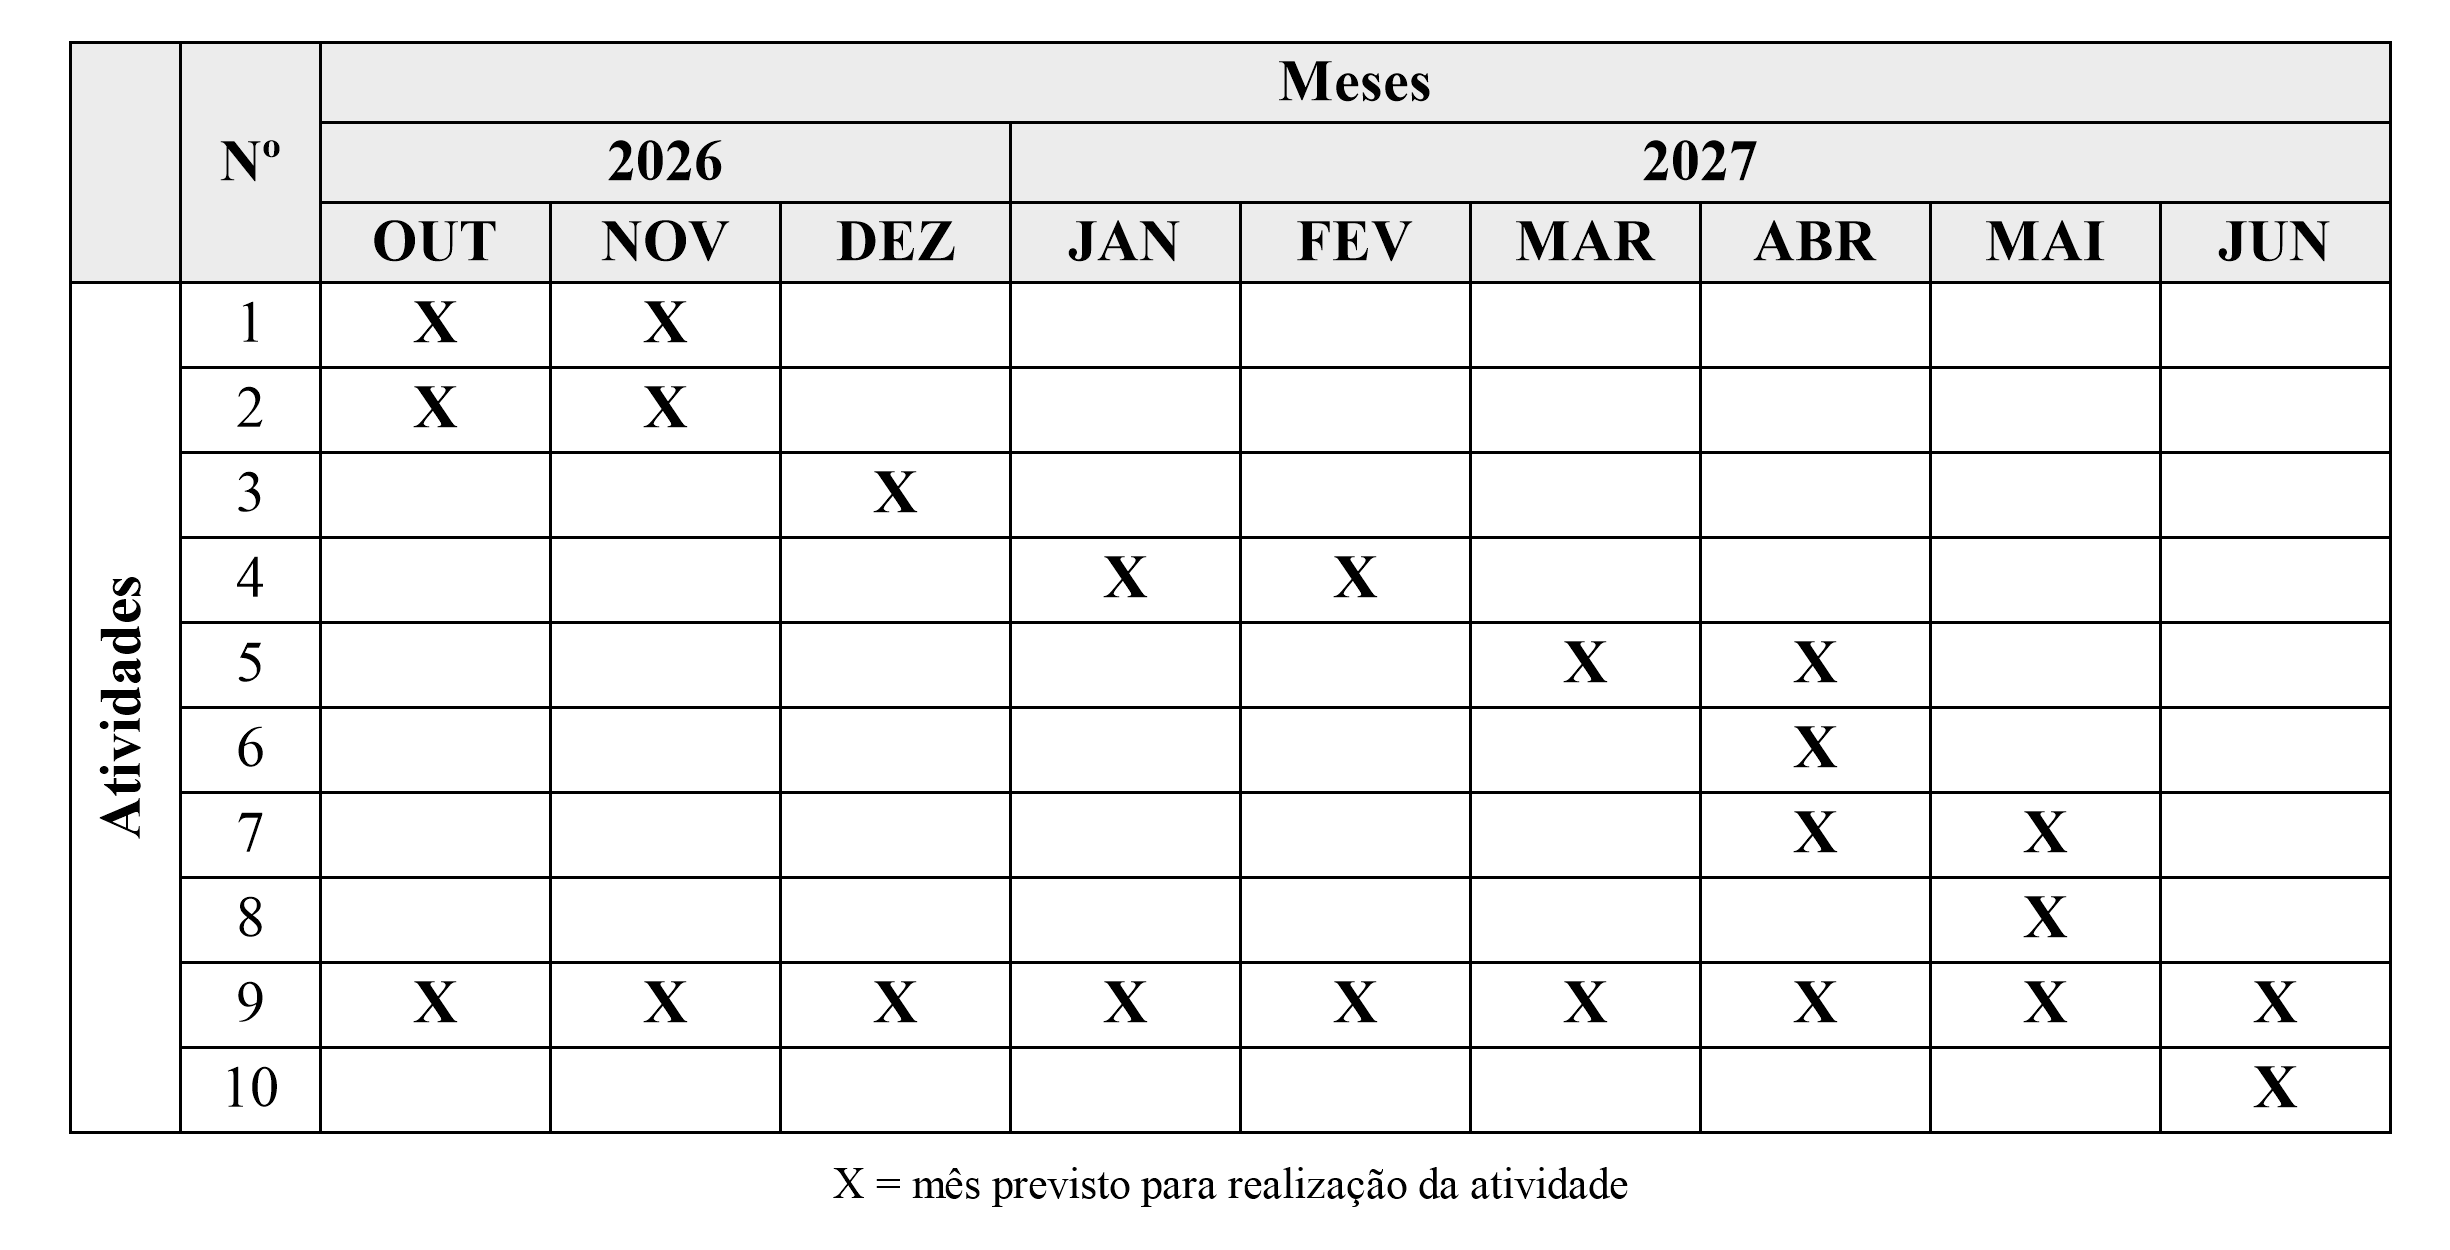
\includegraphics[width=\textwidth]{imagens/cronograma}
    \par\smallskip
    {\footnotesize Fonte: Elaborado pelos autores (2026).}
\end{figure}
\FloatBarrier

\begin{enumerate}
    \item \textbf{Consolidação do pré-projeto (outubro e novembro de 2026):} uniformizar escopo, requisitos, tecnologias, modelos e conclusões parciais, além de registrar o planejamento da equipe e da avaliação.

    \item \textbf{Desenvolvimento da V0 (outubro e novembro de 2026):} implementar uma prova de conceito de conexão com PostgreSQL, introspecção, preparação de contexto, geração, validação e execução de consultas. Incluir consentimento binário para amostras de até cem registros por tabela, com todas as colunas, e utilizar inicialmente um subconjunto de perguntas de teste.

    \item \textbf{Revisão da V0 e planejamento da V1 (dezembro de 2026):} analisar os resultados iniciais, identificar pendências técnicas, apoiar a escolha do modelo e do provedor de linguagem e organizar o backlog e o fluxo da interface.

    \item \textbf{Desenvolvimento do núcleo da V1 (janeiro e fevereiro de 2027):} integrar conexão, consentimento, contexto, geração de SQL, validação, execução com credenciais de leitura, tratamento de falhas e registro das informações de execução. O fluxo admitirá três tentativas totais, incluindo a inicial.

    \item \textbf{Interface e integração desktop (março e abril de 2027):} desenvolver e integrar a interface com React, Vite e TypeScript, disponibilizando conexão, perguntas e resultados tabulares, e organizar a execução local com Electron e backend em FastAPI.

    \item \textbf{Preparação da avaliação (abril de 2027):} consolidar o banco comercial fictício, as perguntas, as consultas de referência, os resultados esperados e os casos de segurança e falha. Congelar os dados e as amostras utilizados na comparação final.

    \item \textbf{Estabilização e correções da V1 (abril e maio de 2027):} verificar os requisitos obrigatórios, executar testes de integração e corrigir os problemas identificados no fluxo principal e na avaliação.

    \item \textbf{Avaliação comparativa e análise dos resultados (maio de 2027):} executar as perguntas com esquema e com esquema acrescido de amostras, registrar métricas e analisar respostas incorretas, tentativas de correção, custos e limitações.

    \item \textbf{Documentação e acompanhamento (outubro de 2026 a junho de 2027):} atualizar o relatório, as decisões, o backlog, os registros de teste e as evidências do trabalho, com participação dos dois integrantes e maior concentração de Raissa na organização documental.

    \item \textbf{Apresentação e entrega final (junho de 2027):} concluir a discussão dos resultados, revisar o relatório e a V1, preparar os materiais de apresentação e realizar a entrega para avaliação final.
\end{enumerate}

A integração e a conclusão dos requisitos essenciais serão priorizadas antes da etapa final. Maio será reservado principalmente para avaliação e correções, enquanto junho será destinado à consolidação da entrega e à apresentação. As versões V2 e V3 permanecerão como possibilidades de evolução, sem integrar o compromisso obrigatório do cronograma.

\section{Planejamento da Avaliação}

A avaliação técnica será conduzida pelos autores em um banco PostgreSQL fictício do domínio comercial, contendo clientes, produtos, pedidos e itens de pedido. Será preparado um conjunto de trinta perguntas válidas em português, distribuídas entre dez consultas simples, oito agregações, oito consultas com junções e quatro consultas que envolvam significado de negócio. Adicionalmente, serão propostas dez verificações de solicitações proibidas e cinco verificações de falhas operacionais.

Cada pergunta válida terá sua interpretação esperada, uma consulta SQL de referência e o resultado esperado documentados. As perguntas utilizadas para ajustes durante o desenvolvimento serão separadas das utilizadas na avaliação final. O banco incluirá situações que permitam identificar erros, como pedidos cancelados, valores nulos e registros próximos aos limites dos períodos consultados.

Uma resposta será considerada correta quando os dados retornados corresponderem ao resultado esperado, incluindo filtros, valores, agrupamentos e ordenação quando solicitada. A igualdade textual com o SQL de referência não será exigida. Consultas que executem sem erro, mas respondam a uma intenção diferente, serão classificadas como incorretas.

O efeito das amostras será investigado pela comparação entre duas configurações:
\begin{enumerate}
    \item contexto contendo apenas os metadados estruturais do banco;
    \item contexto contendo os mesmos metadados e amostras autorizadas de até cem registros por tabela, incluindo todas as colunas.
\end{enumerate}

O modelo, as instruções, as perguntas, os dados e a política de correção serão mantidos constantes. As amostras serão fixadas para permitir a reprodução da comparação. Prevê-se realizar três execuções por pergunta em cada configuração, totalizando cento e oitenta execuções de solicitações válidas, além das verificações de segurança e falha. Cada execução respeitará o limite de três tentativas totais.

Serão registradas a taxa de respostas corretas na primeira tentativa e após as correções, a taxa de execução SQL bem-sucedida, a quantidade de tentativas, a latência e, quando disponíveis, o consumo de tokens e o custo estimado. Os resultados serão apresentados por configuração e grupo de perguntas. Os casos de segurança e falha serão contabilizados separadamente.

Como metas preliminares para discussão com o orientador, propõem-se:
\begin{itemize}
    \item pelo menos 80\% de respostas corretas às perguntas válidas na configuração com amostras, considerando até três tentativas totais;
    \item pelo menos 90\% de solicitações válidas com execução SQL bem-sucedida nessa configuração, independentemente da correção semântica;
    \item nenhuma alteração do banco nas dez verificações de solicitações proibidas;
    \item encerramento controlado nas cinco verificações de falhas operacionais;
    \item ausência de envio de registros ao modelo quando o consentimento for recusado;
    \item realização do fluxo principal pela interface gráfica, sem utilização de terminal pelo usuário.
\end{itemize}

Essas metas deverão ser revisadas com o orientador antes da avaliação final e não constituem critérios oficiais da banca. A configuração sem amostras será avaliada separadamente, sem pressupor que a inclusão de registros necessariamente melhore o desempenho. A meta de latência e os limites de custo serão definidos após as medições da V0.

A avaliação pelos professores considerará a coerência da proposta, a demonstração do sistema, a documentação e as evidências apresentadas. Essa participação não será tratada como um estudo de usabilidade com usuários finais.

% Orientação do template: manter este capítulo em GPD1 e GPD2.
% Para a versão da banca final, removê-lo ou transferi-lo para um apêndice.








% ---------------------------------------------------------------------------------
%                                 ELEMENTOS PÓS-TEXTUAIS
% ---------------------------------------------------------------------------------
\postextual


% ----------------------------------------------------------
% Referências bibliográficas
% ----------------------------------------------------------
\bibliography{referencias}


% ----------------------------------------------------------
% Glossário
% ----------------------------------------------------------
%
% Consulte o manual da classe abntex2 para orientações sobre o glossário.
%
%\glossary


% ----------------------------------------------------------
% Apêndices
% ----------------------------------------------------------
% Texto ou documento elaborado pelo autor, a fim de complementar sua argumentação, sem prejuízo da unidade nuclear do trabalho.

% ---
% Inicia os apêndices
% ---
\begin{apendicesenv}
	
	% Imprime uma página indicando o início dos apêndices
	\partapendices
	
	% ----------------------------------------------------------
	\chapter{Modelo de Requisitos do Sistema}
	% ----------------------------------------------------------
	
\label{ap:requisitos}

Este apêndice apresenta a descrição textual dos requisitos do sistema e o modelo de casos de uso da versão V1 (MVP). Estão organizados os atores envolvidos, as regras de negócio que orientam o comportamento da aplicação, os casos de uso com suas descrições e a rastreabilidade entre requisitos, casos de uso e incrementos. Os requisitos funcionais (RF) e não funcionais (RNF) referenciados estão definidos na Seção~\ref{sec:requisitos}.

\section{Atores}
\label{ap:atores}

O Quadro~\ref{qua:atores} apresenta os atores que interagem com o sistema.

\begin{quadro}[htb]
    \caption{Atores do sistema}
    \label{qua:atores}
    \begin{tabular}{|p{3.2cm}|p{2.6cm}|p{8.4cm}|}
        \hline
        \textbf{Ator} & \textbf{Tipo} & \textbf{Descrição} \\ \hline
        Usuário & Primário & Pessoa que conhece o contexto dos dados, mas não necessariamente domina SQL. Configura a conexão, decide sobre o uso de amostras, formula perguntas e visualiza os resultados. \\ \hline
        Provedor de IA & Secundário (externo) & Serviço de modelo de linguagem (por exemplo, OpenAI ou DeepSeek) que interpreta a solicitação e gera ou corrige a consulta SQL a partir do contexto recebido. \\ \hline
        Banco PostgreSQL & Secundário (externo) & Banco de dados do usuário, acessado com as credenciais informadas, do qual são extraídos os metadados estruturais, as amostras autorizadas e os resultados das consultas. \\ \hline
    \end{tabular}
    \legend{Fonte: Elaborado pelos autores (2026).}
\end{quadro}

\section{Regras de Negócio}
\label{ap:regras}

As regras de negócio a seguir complementam os requisitos e delimitam o comportamento esperado da aplicação.

\begin{itemize}
    \item \textbf{RN01 -- Somente leitura:} apenas consultas de leitura, compostas por uma única instrução \texttt{SELECT}, podem ser executadas.
    \item \textbf{RN02 -- Validação independente:} a resposta do modelo de linguagem não é tratada como confiável; toda consulta gerada passa por uma camada de validação sintática e de segurança independente do modelo antes da execução.
    \item \textbf{RN03 -- Comandos bloqueados:} comandos como \texttt{INSERT}, \texttt{UPDATE}, \texttt{DELETE}, \texttt{DROP}, \texttt{ALTER} e \texttt{TRUNCATE}, bem como quaisquer outros capazes de alterar registros ou estruturas, devem ser bloqueados antes da execução.
    \item \textbf{RN04 -- Execução controlada:} as consultas aprovadas são executadas em modo somente leitura sobre o banco informado.
    \item \textbf{RN05 -- Estrutura determinística:} os metadados estruturais (esquemas, tabelas, colunas, tipos, chaves primárias e estrangeiras) são obtidos pelo módulo de introspecção, e não por inferência do modelo de linguagem.
    \item \textbf{RN06 -- Consentimento explícito:} nenhum registro do banco é enviado ao provedor de IA sem autorização explícita do usuário.
    \item \textbf{RN07 -- Limite de amostragem:} quando autorizada, cada amostragem contém no máximo dez registros.
    \item \textbf{RN08 -- Limite de correções:} uma consulta permitida que falhe pode ser reenviada ao modelo para correção em até três tentativas; esgotadas as tentativas, a operação é encerrada com informação ao usuário.
    \item \textbf{RN09 -- Alcance definido pelas credenciais:} o sistema considera apenas as estruturas acessíveis às credenciais fornecidas pelo usuário.
    \item \textbf{RN10 -- Rastreabilidade técnica:} latência, erros, número de tentativas e execução das consultas são registrados para apoiar a avaliação do sistema.
\end{itemize}

\section{Casos de Uso}
\label{ap:casos-uso}

A Figura~\ref{fig:casos-uso} apresenta o diagrama de casos de uso do MVP e o Quadro~\ref{qua:casos-uso} relaciona cada caso de uso aos requisitos que ele atende.

\begin{figure}[htb]
    \centering
    \caption{Diagrama de casos de uso do MVP (V1)}
    \label{fig:casos-uso}
    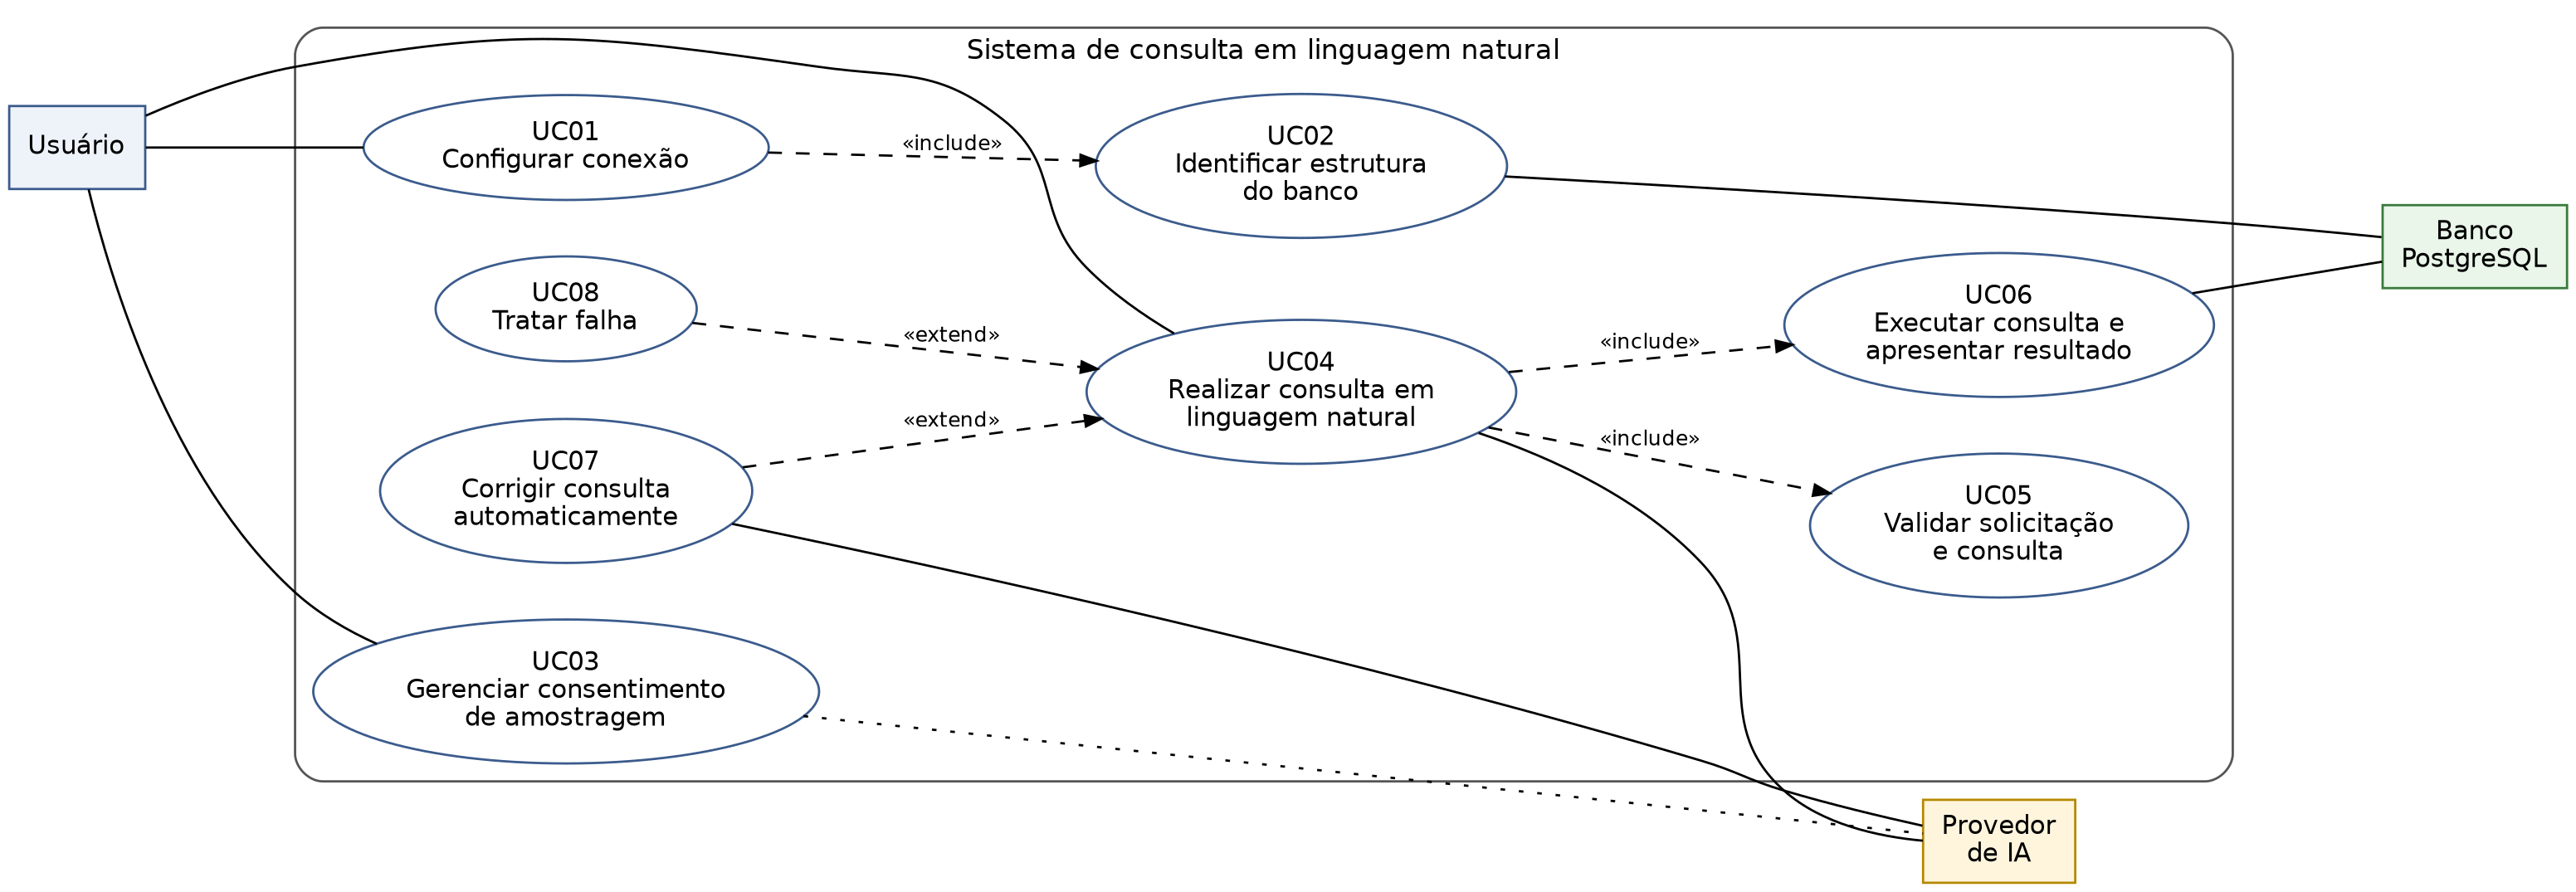
\includegraphics[width=\textwidth]{imagens/casos_de_uso.png}
    \legend{Fonte: Elaborado pelos autores (2026).}
\end{figure}

\begin{quadro}[htb]
    \caption{Casos de uso e requisitos atendidos}
    \label{qua:casos-uso}
    \begin{tabular}{|p{1.5cm}|p{6.2cm}|p{3.0cm}|p{3.5cm}|}
        \hline
        \textbf{Código} & \textbf{Caso de uso} & \textbf{Requisitos} & \textbf{Ator(es)} \\ \hline
        UC01 & Configurar conexão com o banco & RF01 & Usuário \\ \hline
        UC02 & Identificar estrutura do banco & RF02, RF03 & Banco PostgreSQL \\ \hline
        UC03 & Gerenciar consentimento de amostragem & RF04, RF05 & Usuário, Provedor de IA \\ \hline
        UC04 & Realizar consulta em linguagem natural & RF06, RF08 & Usuário, Provedor de IA \\ \hline
        UC05 & Validar solicitação e consulta & RF07, RNF01 & (interno) \\ \hline
        UC06 & Executar consulta e apresentar resultado & RF09, RF10 & Banco PostgreSQL \\ \hline
        UC07 & Corrigir consulta automaticamente & RF11 & Provedor de IA \\ \hline
        UC08 & Tratar falha & RF12, RNF06 & Usuário \\ \hline
    \end{tabular}
    \legend{Fonte: Elaborado pelos autores (2026).}
\end{quadro}

\subsection{UC01 -- Configurar conexão com o banco}

\begin{description}
    \item[Objetivo:] permitir que o usuário informe os dados de acesso a um banco PostgreSQL.
    \item[Ator:] Usuário.
    \item[Pré-condição:] a aplicação está em execução.
    \item[Pós-condição:] conexão estabelecida e estrutura do banco identificada (UC02).
\end{description}

\textbf{Fluxo principal:}
\begin{enumerate}
    \item O usuário informa os dados de conexão (servidor, porta, banco, usuário e senha).
    \item O sistema tenta estabelecer a conexão.
    \item O sistema aciona a identificação da estrutura do banco (UC02).
    \item O sistema informa que o banco está pronto para receber perguntas.
\end{enumerate}

\textbf{Fluxo alternativo:} se a conexão falhar (dados incorretos ou banco inacessível), o sistema informa o erro ao usuário e permite corrigir os dados (RNF06).

\subsection{UC02 -- Identificar estrutura do banco}

\begin{description}
    \item[Objetivo:] levantar automaticamente a estrutura acessível do banco, sem depender do modelo de linguagem.
    \item[Ator:] Banco PostgreSQL.
    \item[Pré-condição:] conexão estabelecida (UC01).
    \item[Pós-condição:] representação estruturada com esquemas, tabelas, colunas, tipos, chaves primárias e estrangeiras disponível para composição do contexto.
\end{description}

\textbf{Fluxo principal:}
\begin{enumerate}
    \item O sistema lista os esquemas acessíveis às credenciais informadas (RF02).
    \item Para cada esquema, o sistema obtém tabelas, colunas, tipos de dados, chaves primárias e chaves estrangeiras (RF03).
    \item O sistema organiza as informações em uma representação estruturada.
\end{enumerate}

\subsection{UC03 -- Gerenciar consentimento de amostragem}

\begin{description}
    \item[Objetivo:] permitir que o usuário autorize ou recuse o envio de amostras de registros ao provedor de IA.
    \item[Ator:] Usuário.
    \item[Pré-condição:] estrutura do banco identificada (UC02).
    \item[Pós-condição:] preferência de amostragem registrada para a sessão.
\end{description}

\textbf{Fluxo principal:}
\begin{enumerate}
    \item O sistema informa que as amostras podem conter dados sensíveis e solicita autorização explícita (RF04).
    \item O usuário autoriza a utilização das amostras.
    \item Quando necessário, o sistema coleta amostras de, no máximo, dez registros por operação (RF05) e as inclui no contexto.
\end{enumerate}

\textbf{Fluxo alternativo:} se o usuário recusar, nenhum registro é lido para composição do contexto e o sistema opera apenas com os metadados estruturais (RNF03).

\subsection{UC04 -- Realizar consulta em linguagem natural}

\begin{description}
    \item[Objetivo:] obter dados do banco a partir de uma pergunta escrita em linguagem natural.
    \item[Atores:] Usuário e Provedor de IA.
    \item[Pré-condição:] banco conectado e estrutura identificada.
    \item[Pós-condição:] resultado apresentado em formato tabular, ou falha informada de forma controlada.
\end{description}

\textbf{Fluxo principal:}
\begin{enumerate}
    \item O usuário digita uma pergunta em linguagem natural (RF06).
    \item O sistema prepara o contexto com a estrutura do banco e, se autorizadas, as amostras.
    \item O sistema verifica se a solicitação é compatível com o escopo de leitura (UC05).
    \item O sistema solicita ao provedor de IA a geração da consulta SQL (RF08).
    \item O sistema valida a consulta gerada (UC05).
    \item O sistema executa a consulta aprovada e apresenta o resultado em tabela (UC06).
\end{enumerate}

\textbf{Fluxos alternativos:}
\begin{enumerate}
    \item[A1.] \emph{Solicitação incompatível:} se a pergunta exigir inserção, atualização, exclusão ou alteração estrutural, o sistema não prossegue para a execução e informa o motivo ao usuário (RF07).
    \item[A2.] \emph{Consulta reprovada na validação:} a consulta não é executada; o sistema pode solicitar nova geração dentro do limite de tentativas (UC07) ou, esgotado o limite, tratar a falha (UC08).
    \item[A3.] \emph{Erro de geração ou execução:} o sistema aciona a correção automática (UC07).
\end{enumerate}

\subsection{UC05 -- Validar solicitação e consulta}

Caso de uso incluído em UC04. O sistema verifica a intenção da pergunta (RF07) e, após a geração, analisa a consulta produzida por uma camada de validação independente do modelo, aprovando apenas uma instrução \texttt{SELECT} e bloqueando comandos de escrita ou de alteração estrutural (RN01 a RN03; RNF01).

\subsection{UC06 -- Executar consulta e apresentar resultado}

Caso de uso incluído em UC04. O sistema executa a consulta aprovada em modo somente leitura (RF09; RN04), processa o resultado e o apresenta ao usuário em formato tabular na interface gráfica (RF10), registrando latência e demais informações de execução (RNF07).

\subsection{UC07 -- Corrigir consulta automaticamente}

Caso de uso que estende UC04. Quando uma consulta permitida falha na geração ou na execução, o sistema envia o erro ao provedor de IA e obtém uma nova versão da consulta, repetindo o processo em até três tentativas (RF11; RN08). Cada tentativa é registrada para fins de avaliação (RN10).

\subsection{UC08 -- Tratar falha}

Caso de uso que estende UC04. Esgotado o limite de tentativas, ou diante de falhas de conexão ou de comunicação com o provedor de IA, o sistema encerra a operação de maneira controlada e informa a falha ao usuário, sem executar consultas não aprovadas (RF12; RNF06).

\section{Rastreabilidade dos Requisitos}
\label{ap:rastreabilidade}

O Quadro~\ref{qua:rastreabilidade} relaciona os requisitos funcionais aos casos de uso e aos incrementos em que são implementados. O fluxo essencial é validado tecnicamente na V0 e integrado à interface gráfica na V1.

\begin{quadro}[htb]
    \caption{Rastreabilidade dos requisitos funcionais}
    \label{qua:rastreabilidade}
    \begin{tabular}{|p{1.4cm}|p{7.2cm}|p{2.2cm}|p{2.8cm}|}
        \hline
        \textbf{Req.} & \textbf{Descrição resumida} & \textbf{Caso de uso} & \textbf{Incremento} \\ \hline
        RF01 & Conexão com banco de dados & UC01 & V0 e V1 \\ \hline
        RF02 & Identificação de esquemas & UC02 & V0 e V1 \\ \hline
        RF03 & Introspecção estrutural & UC02 & V0 e V1 \\ \hline
        RF04 & Consentimento para amostragem & UC03 & V1 \\ \hline
        RF05 & Limitação das amostras & UC03 & V1 \\ \hline
        RF06 & Entrada em linguagem natural & UC04 & V0 e V1 \\ \hline
        RF07 & Validação da intenção & UC04, UC05 & V0 e V1 \\ \hline
        RF08 & Geração de consulta SQL & UC04 & V0 e V1 \\ \hline
        RF09 & Execução da consulta & UC06 & V0 e V1 \\ \hline
        RF10 & Apresentação do resultado & UC06 & V0 e V1 \\ \hline
        RF11 & Correção automática de consultas & UC07 & V1 \\ \hline
        RF12 & Tratamento de falha & UC08 & V1 \\ \hline
    \end{tabular}
    \legend{Fonte: Elaborado pelos autores (2026).}
\end{quadro}

\section{Critérios de Verificação dos Requisitos Não Funcionais}
\label{ap:criterios-rnf}

O Quadro~\ref{qua:criterios-rnf} indica como cada requisito não funcional será verificado durante a validação do sistema.

\begin{quadro}[htb]
    \caption{Critérios de verificação dos requisitos não funcionais}
    \label{qua:criterios-rnf}
    \begin{tabular}{|p{1.7cm}|p{4.0cm}|p{8.5cm}|}
        \hline
        \textbf{Req.} & \textbf{Requisito} & \textbf{Forma de verificação} \\ \hline
        RNF01 & Segurança & Conjunto de solicitações e consultas proibidas; medição da taxa de bloqueio correto. \\ \hline
        RNF02 & Privacidade & Inspeção do contexto enviado ao provedor, verificando a ausência de registros sem consentimento. \\ \hline
        RNF03 & Independência da amostragem & Execução do fluxo principal com a amostragem recusada. \\ \hline
        RNF04 & Modularidade & Revisão da arquitetura quanto à separação entre introspecção, contexto, geração, validação, execução e apresentação. \\ \hline
        RNF05 & Baixo acoplamento ao modelo & Substituição do provedor de IA sem alteração dos demais módulos. \\ \hline
        RNF06 & Tratamento de erros & Simulação de falhas de conexão, de provedor, de geração e de execução. \\ \hline
        RNF07 & Observabilidade & Verificação dos registros de latência, erros, tentativas e execuções. \\ \hline
        RNF08 & Usabilidade & Execução do fluxo principal pela interface desktop, sem uso de terminal ou código-fonte. \\ \hline
    \end{tabular}
    \legend{Fonte: Elaborado pelos autores (2026).}
\end{quadro}
	
	
	
	% ----------------------------------------------------------
	\chapter{Modelo Estrutural do Sistema}
	% ----------------------------------------------------------

  \label{ap:estrutural}

Este apêndice apresenta o modelo estrutural do sistema por meio de diagramas de classes da UML. Optou-se por dois diagramas complementares: o modelo de domínio, que representa as informações manipuladas pela aplicação, e o modelo de módulos do backend, que representa as classes responsáveis por cada etapa do fluxo descrito na Seção~\ref{sec:visao-geral}. Os nomes seguem a nomenclatura de implementação prevista e podem ser refinados durante o desenvolvimento.

\section{Modelo de Domínio}
\label{ap:dominio}

A Figura~\ref{fig:dominio} apresenta as principais classes de domínio. A estrutura do banco é obtida a partir de uma conexão e composta por esquemas, tabelas, colunas e chaves estrangeiras, obtidos de forma determinística pelo módulo de introspecção. As amostras de registros são opcionais e associadas às tabelas somente quando o usuário as autoriza. O contexto de consulta reúne a estrutura, as amostras eventuais e a pergunta, e serve de base para a geração da consulta SQL, que passa por validação e, quando aprovada, produz um resultado.

\begin{figure}[htb]
    \centering
    \caption{Diagrama de classes -- modelo de domínio}
    \label{fig:dominio}
    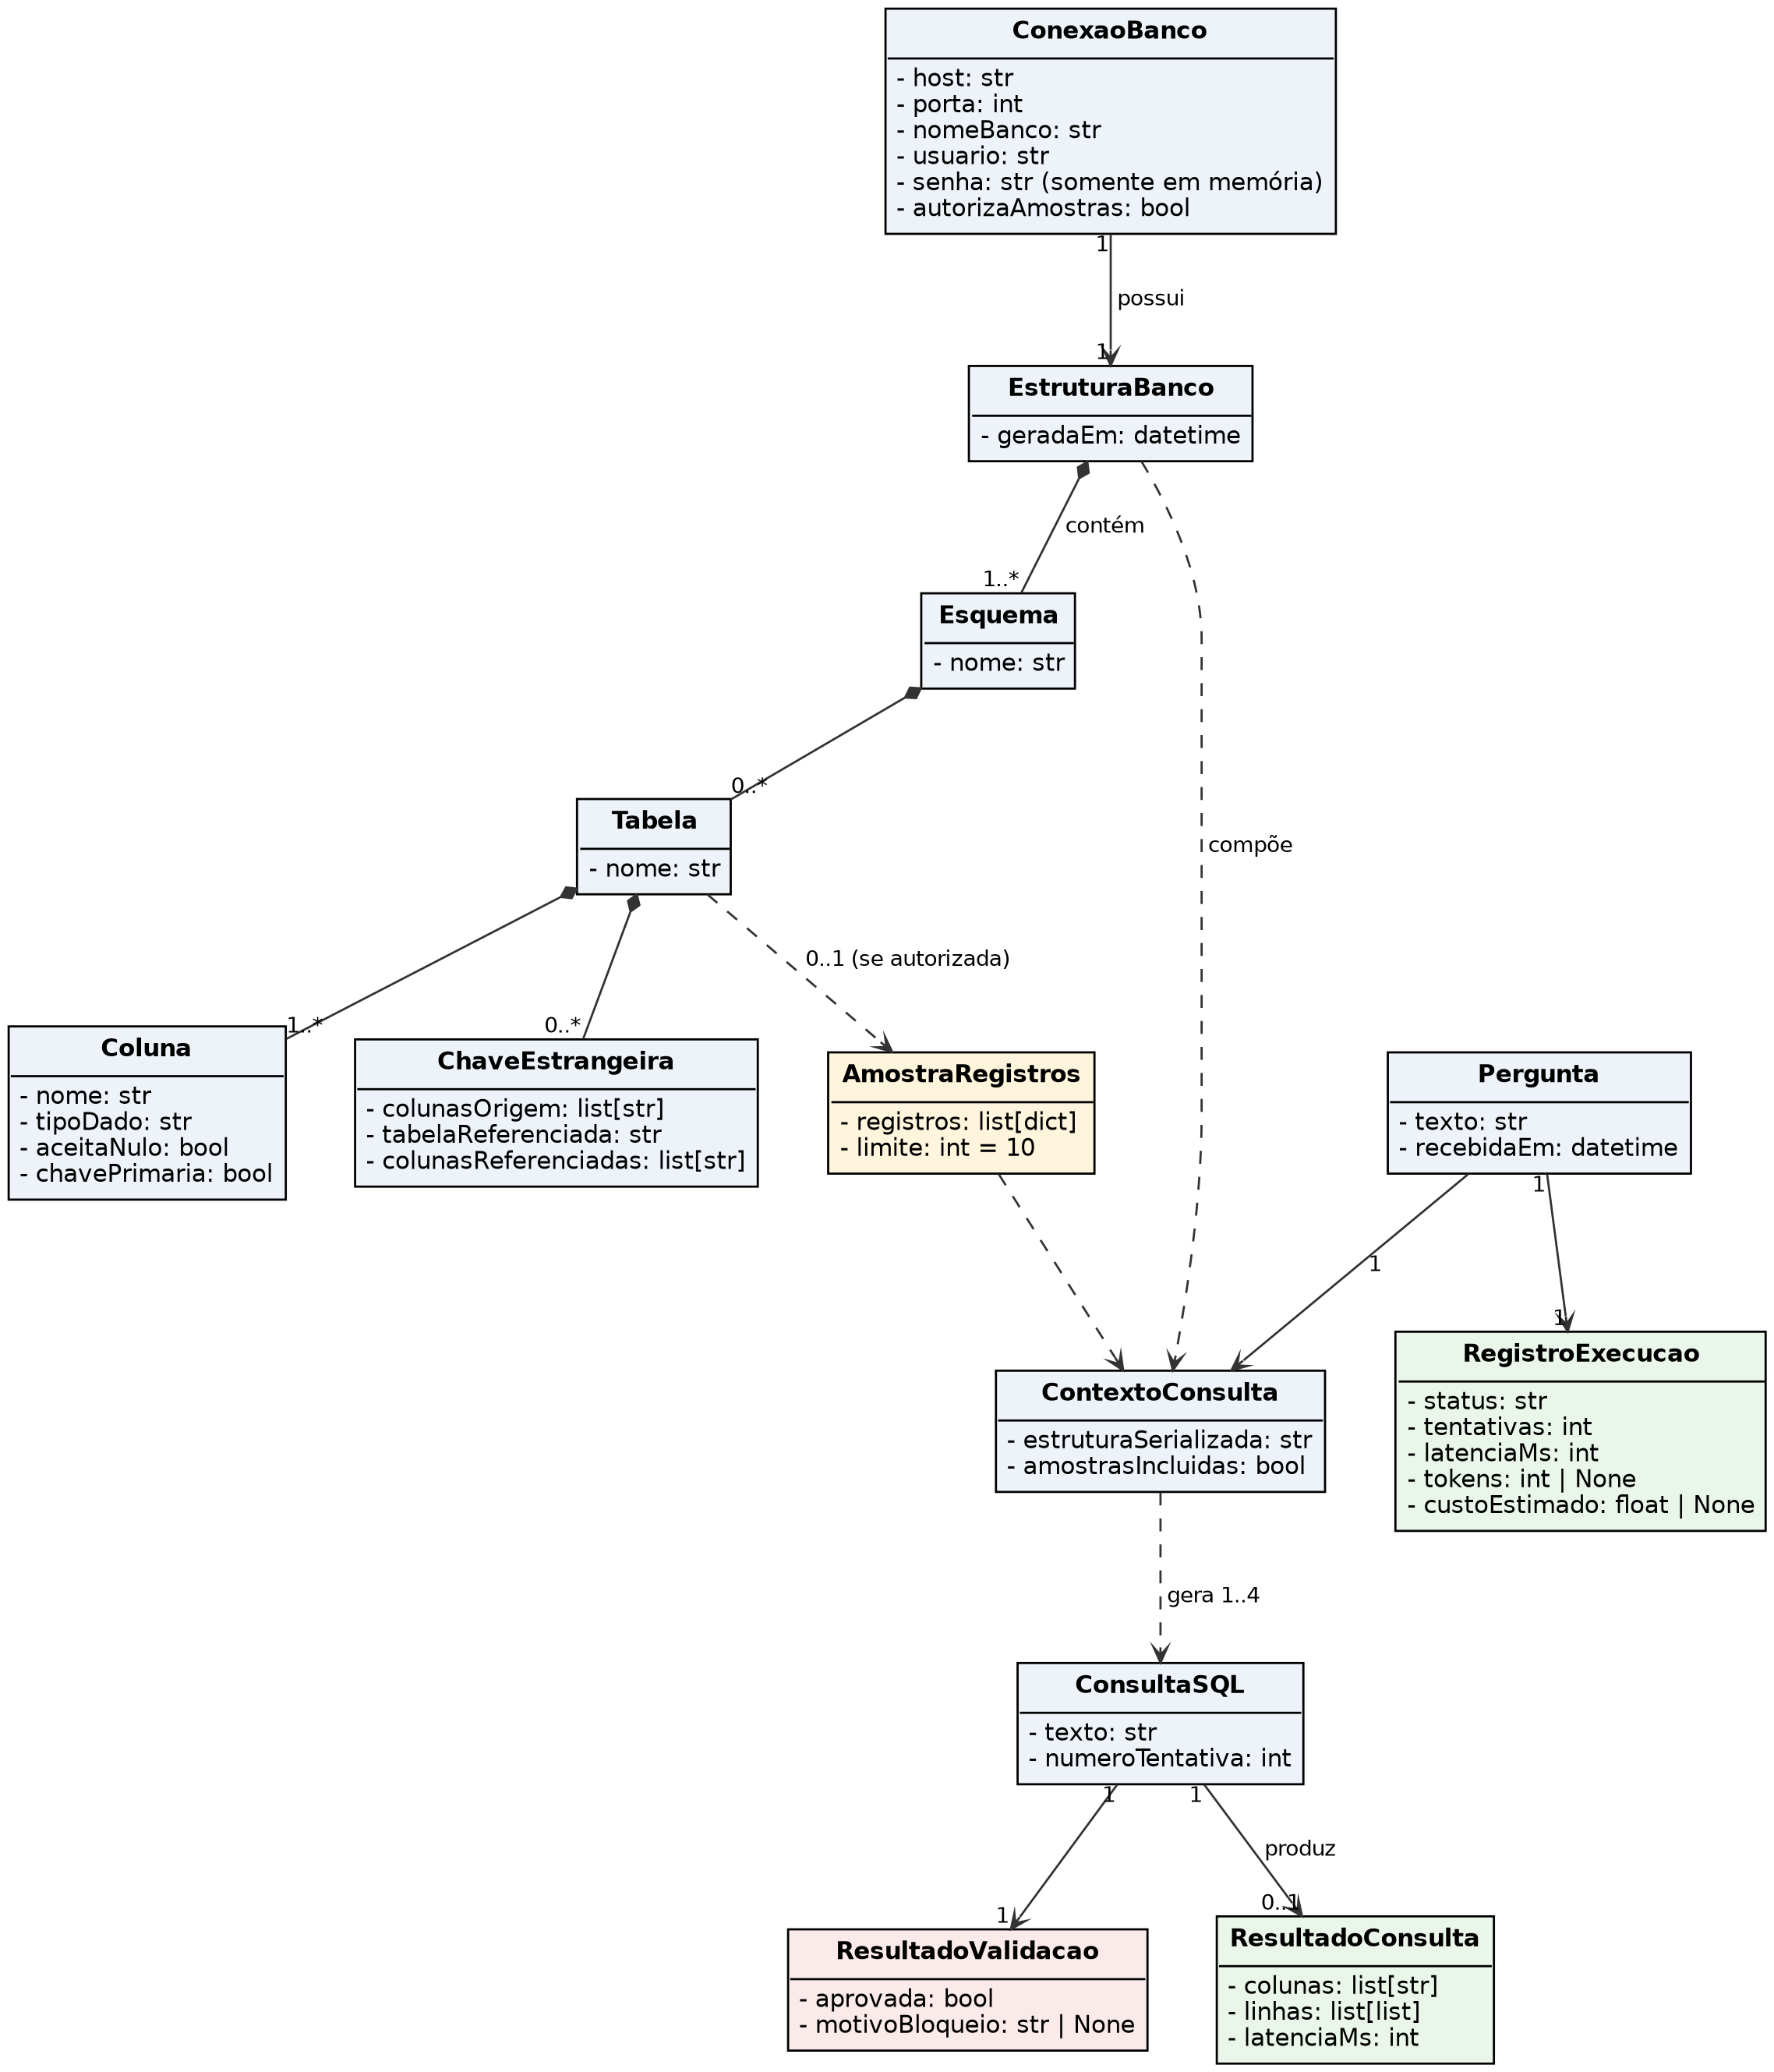
\includegraphics[width=\textwidth]{imagens/diagrama_classes_dominio.png}
    \legend{Fonte: Elaborado pelos autores (2026).}
\end{figure}

O Quadro~\ref{qua:classes-dominio} descreve a responsabilidade de cada classe.

\begin{quadro}[htb]
    \caption{Classes do modelo de domínio}
    \label{qua:classes-dominio}
    \begin{tabular}{|p{3.6cm}|p{10.6cm}|}
        \hline
        \textbf{Classe} & \textbf{Responsabilidade} \\ \hline
        ConexaoBanco & Dados de acesso ao PostgreSQL informados pelo usuário e sua decisão sobre o uso de amostras (RF01, RF04). A senha é mantida apenas em memória durante a sessão. \\ \hline
        EstruturaBanco & Representação estruturada de tudo o que foi identificado na introspecção (RF02, RF03). \\ \hline
        Esquema, Tabela, Coluna & Elementos estruturais do banco, incluindo tipo de dado, aceitação de nulos e indicação de chave primária. \\ \hline
        ChaveEstrangeira & Relacionamento entre tabelas, usado para que a geração de SQL reconheça junções possíveis. \\ \hline
        AmostraRegistros & Conjunto opcional de registros, limitado a dez por amostragem (RF05), incluído no contexto somente com consentimento. \\ \hline
        Pergunta & Solicitação em linguagem natural formulada pelo usuário (RF06). \\ \hline
        ContextoConsulta & Contexto enviado ao provedor de IA, composto pela estrutura, pelas amostras (se houver) e pela pergunta. \\ \hline
        ConsultaSQL & Consulta gerada pelo modelo, com indicação do número da tentativa, de modo a controlar as correções (RF11). \\ \hline
        ResultadoValidacao & Resultado da análise de segurança: consulta aprovada ou bloqueada, com o motivo (RF07, RNF01). \\ \hline
        ResultadoConsulta & Colunas, linhas e latência da consulta executada (RF09, RF10). \\ \hline
        RegistroExecucao & Informações de observabilidade de cada solicitação: estado final, tentativas, latência e, quando disponíveis, tokens e custo estimado (RNF07). \\ \hline
    \end{tabular}
    \legend{Fonte: Elaborado pelos autores (2026).}
\end{quadro}

\section{Modelo de Módulos do Backend}
\label{ap:modulos}

A Figura~\ref{fig:servicos} apresenta as classes de serviço do backend em Python e FastAPI. Cada uma concentra uma etapa do fluxo, atendendo ao requisito de modularidade (RNF04). O \texttt{OrquestradorConsulta} coordena a sequência de etapas e é o único componente que conhece a ordem do fluxo. A comunicação com o provedor de inteligência artificial ocorre exclusivamente por meio da interface \texttt{ProvedorLLM}, implementada por classes específicas de cada provedor, o que permite a substituição do modelo sem alterar as demais classes (RNF05).

\begin{figure}[htb]
    \centering
    \caption{Diagrama de classes -- módulos do backend}
    \label{fig:servicos}
    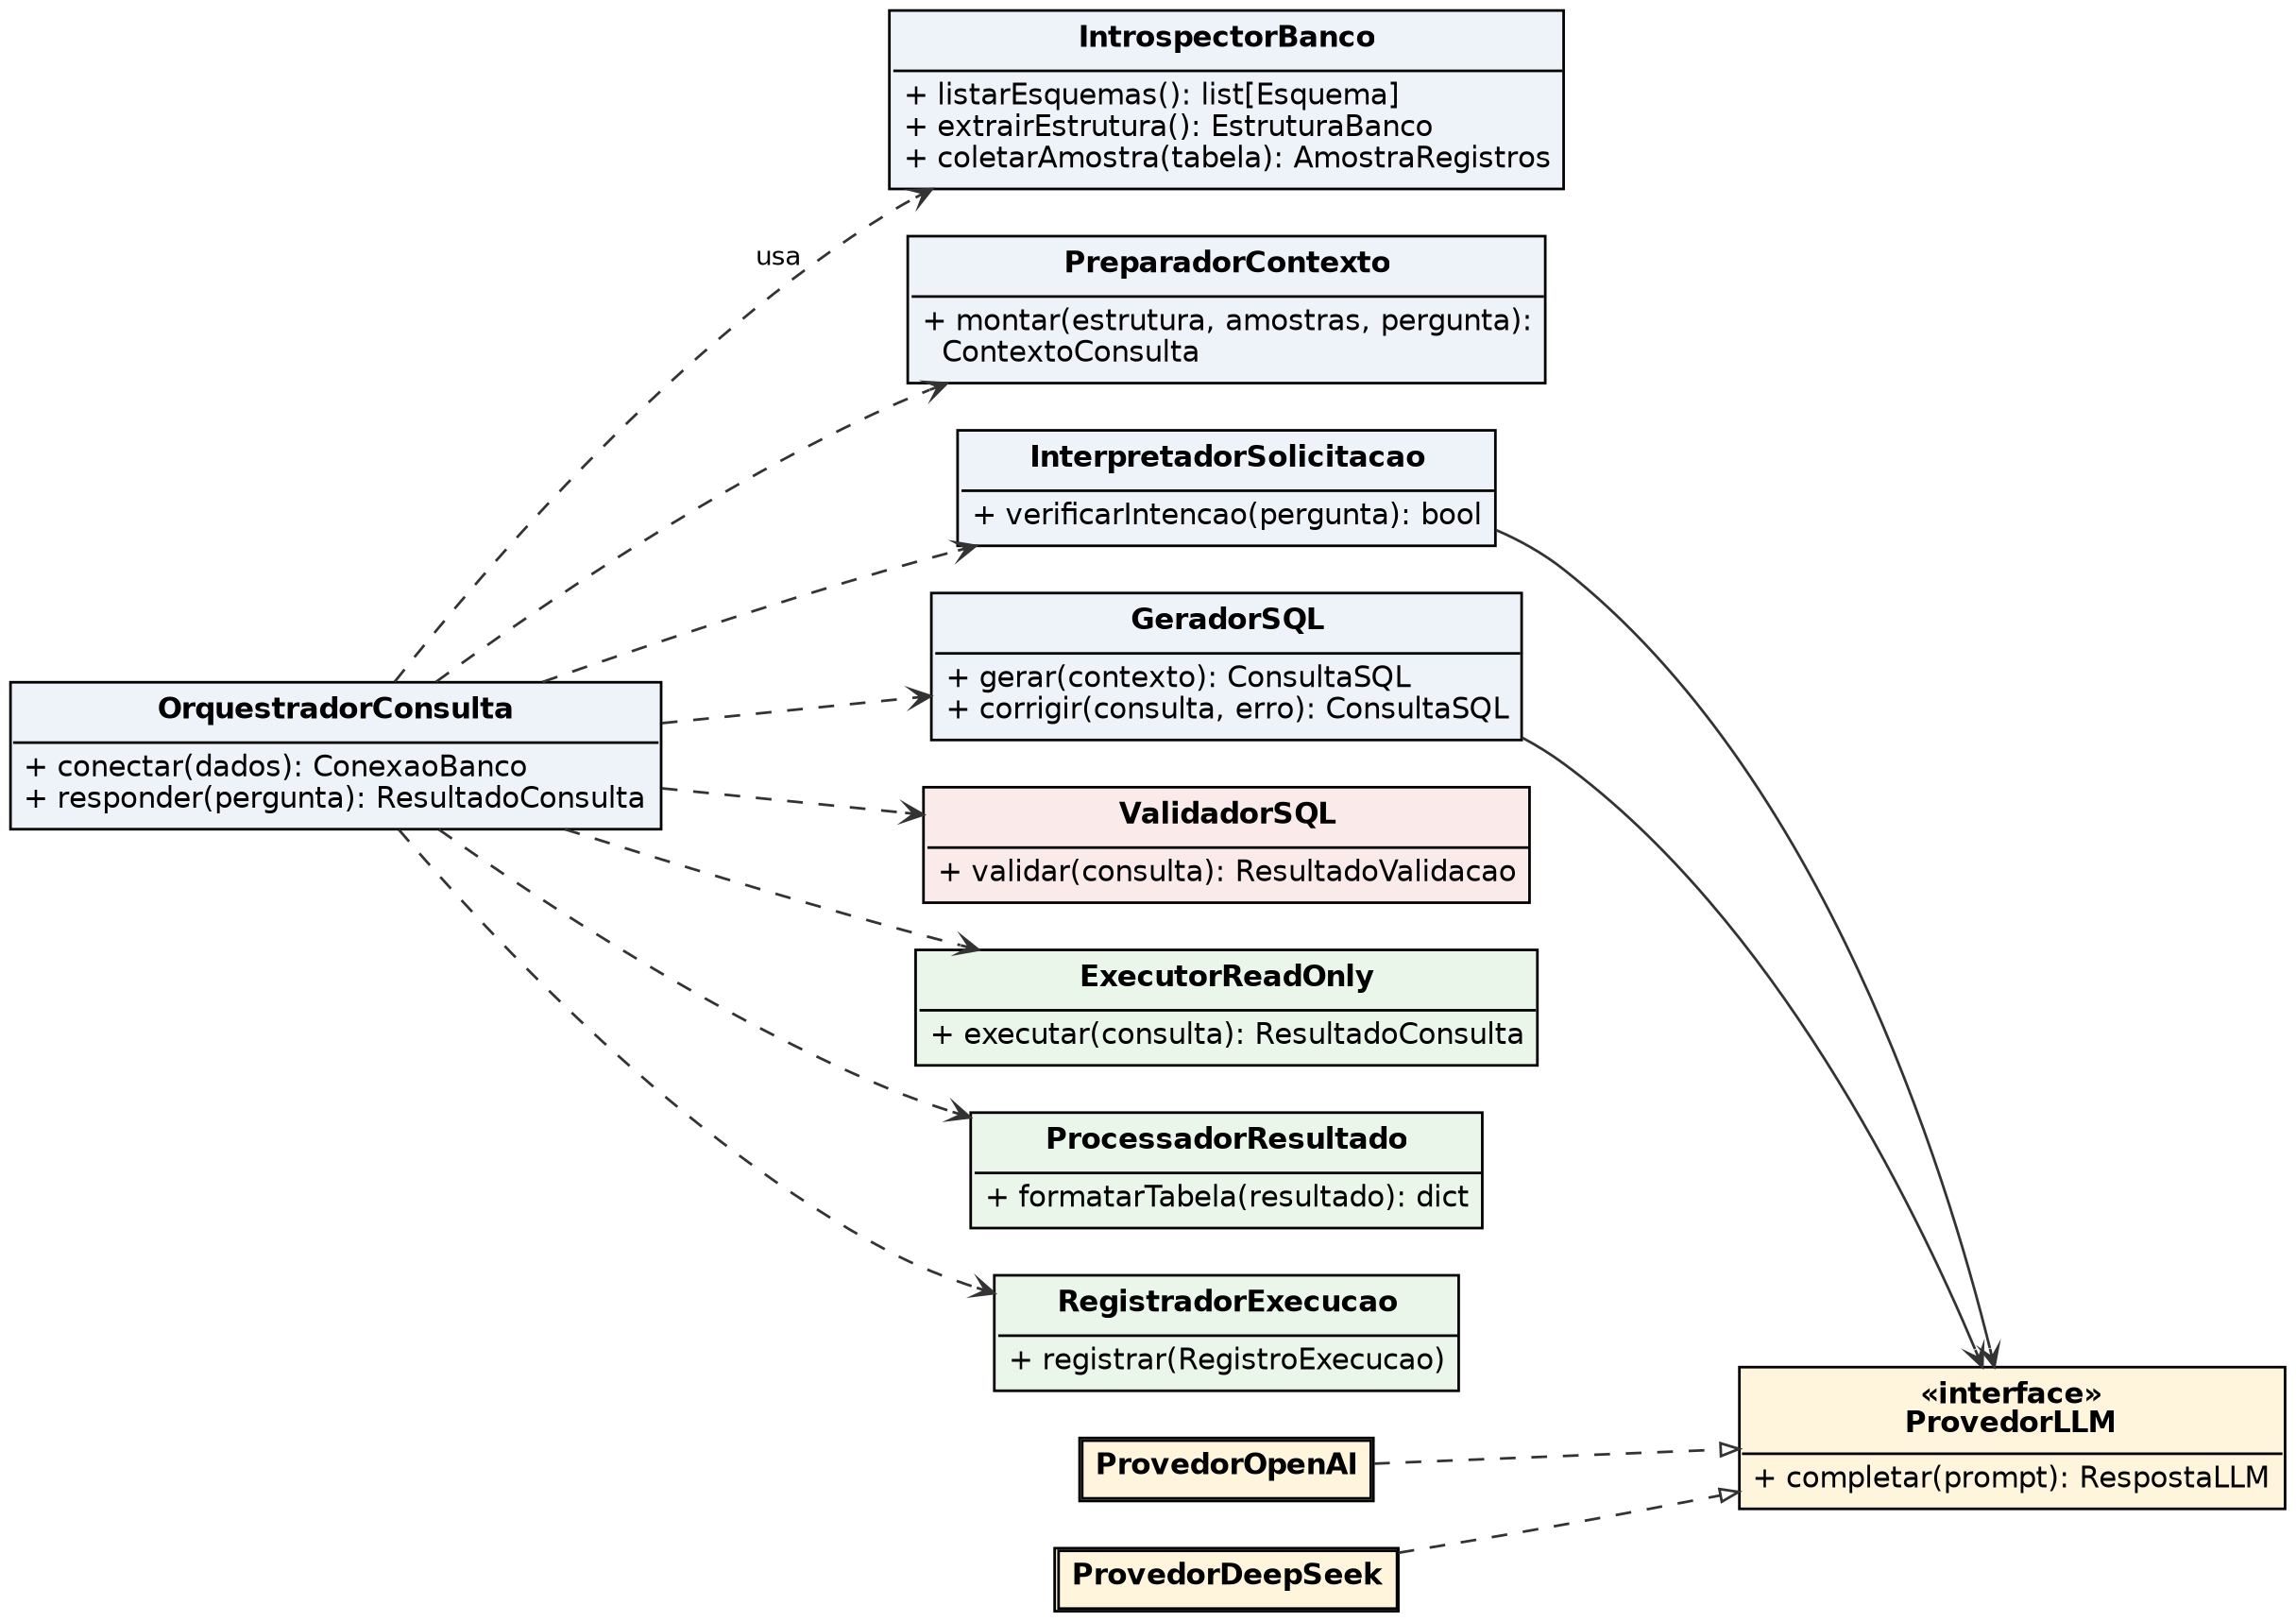
\includegraphics[width=\textwidth]{imagens/diagrama_classes_servicos.png}
    \legend{Fonte: Elaborado pelos autores (2026).}
\end{figure}

\begin{quadro}[htb]
    \caption{Classes de serviço do backend}
    \label{qua:classes-servicos}
    \begin{tabular}{|p{4.0cm}|p{10.2cm}|}
        \hline
        \textbf{Classe} & \textbf{Responsabilidade} \\ \hline
        OrquestradorConsulta & Coordena o fluxo completo, do recebimento da pergunta à entrega do resultado, incluindo o controle do limite de tentativas de correção. \\ \hline
        IntrospectorBanco & Módulo de descoberta (\textit{crawler}): lista esquemas, extrai a estrutura e, quando autorizado, coleta as amostras. \\ \hline
        PreparadorContexto & Monta o contexto enviado ao modelo a partir da estrutura, das amostras e da pergunta. \\ \hline
        InterpretadorSolicitacao & Identifica solicitações incompatíveis com o escopo de leitura (RF07). \\ \hline
        GeradorSQL & Gera a consulta SQL e, em caso de erro, solicita sua correção (RF08, RF11). \\ \hline
        ProvedorLLM (interface) & Contrato de comunicação com o modelo de linguagem, implementado por ProvedorOpenAI e ProvedorDeepSeek. \\ \hline
        ValidadorSQL & Camada de guardrails independente do modelo: aprova apenas consultas de leitura e bloqueia as demais (RNF01). \\ \hline
        ExecutorReadOnly & Executa a consulta aprovada em modo somente leitura (RF09). \\ \hline
        ProcessadorResultado & Converte o resultado para o formato entregue à interface (RF10). \\ \hline
        RegistradorExecucao & Registra latência, erros, tentativas e execuções (RNF07). \\ \hline
    \end{tabular}
    \legend{Fonte: Elaborado pelos autores (2026).}
\end{quadro}

\section{Considerações sobre o Modelo}
\label{ap:consideracoes-modelo}

As classes de domínio serão implementadas como modelos Pydantic, que definem contratos explícitos de entrada e saída da API e validam os dados trocados entre a interface e o backend. O acesso ao PostgreSQL e a introspecção utilizarão o SQLAlchemy. Diagramas complementares de comportamento, arquitetura e dados são apresentados nos apêndices seguintes.

	
	
	
	% ----------------------------------------------------------
	\chapter{Modelo Comportamental do Sistema}
	% ----------------------------------------------------------
   
    Texto de apresentação do Apêndice - Fluxograma ou Diagrama de Sequência ou Diagrama de Estados..
	
	
	
	% ----------------------------------------------------------
	\chapter{Modelo da Arquitetura do Sistema}
	% ----------------------------------------------------------
	
	Texto de apresentação do Apêndice - Diagrama de blocos de alto nível ou Diagrama de Componentes.
	
	
	% ----------------------------------------------------------
	\chapter{Modelo de Dados do Sistema}
	% ----------------------------------------------------------
	
    Texto de apresentação do Apêndice - Modelo Entidade-Relacionamento e Diagrama Entidade-Relacionamento.

    % ----------------------------------------------------------
	\chapter{Outro Apêndice}
	% ----------------------------------------------------------
	
	Texto do Apêndice adicional.



 
\end{apendicesenv}


% ----------------------------------------------------------
% Anexos
% ----------------------------------------------------------
% Texto ou documento não elaborado pelo autor, que serve de fundamentação, comprovação e ilustração.

% ---
% Inicia os anexos
% ---
\begin{anexosenv}
	
	% Imprime uma página indicando o início dos anexos
	\partanexos
	
	% ----------------------------------------------------------
	\chapter{Título do Anexo A}
	% ----------------------------------------------------------
	
	Texto do Anexo A.
	
	
	
	% ----------------------------------------------------------
	\chapter{Título do Anexo B}
	% ----------------------------------------------------------
	
	Texto do Anexo B.
	
	
	
	% ----------------------------------------------------------
	\chapter{Título do Anexo C}
	% ----------------------------------------------------------
	
	Texto do Anexo C.
	
	
	
	% ----------------------------------------------------------
	\chapter{Título do Anexo D}
	% ----------------------------------------------------------
	
	Texto do Anexo D.
	
	
	
	% ----------------------------------------------------------
	\chapter{Título do Anexo E}
	% ----------------------------------------------------------
	
	Texto do Anexo E.
	
	
	
\end{anexosenv}


%---------------------------------------------------------------------
% ÍNDICE REMISSIVO
%---------------------------------------------------------------------

%\phantompart

%\printindex


\end{document}
